\documentclass[a4paper, 14pt, oneside]{Thesis}
\usepackage{ulem}
\usepackage[square, numbers, comma, sort&compress]{natbib}  % Use the "Natbib" style for the references in the Bibliography
\usepackage{verbatim} 
\usepackage{pslatex} %To set the font as Times New Roman
\usepackage{amsbsy} 
\usepackage{amsfonts}
\usepackage{graphicx}
\usepackage{dcolumn}
\usepackage{amsmath}
\usepackage{latexsym}
\usepackage{amssymb}
\usepackage{epsfig}
\usepackage{verbatim} 
\usepackage{epsfig,graphics}
\usepackage{subfigure}
\usepackage{tikz}
\usepackage{float}
\usepackage{algorithm}
\usepackage{algpseudocode}
\usepackage{subcaption}
\usepackage{placeins}  % For FloatBarrier

%\usepackage{fancyhdr}
%\usepackage{lipsum}

%To have 1. instead of [1] in the bibliographic entry
\makeatletter
\renewcommand\@biblabel[1]{#1.}
\makeatother

% To remove hyphenation
\tolerance=1
\emergencystretch=\maxdimen
\hyphenpenalty=10000
\hbadness=10000
%
%----To make sure the page numbers are in the top middle of each page.
\fancypagestyle{Thesis}{
\fancyhf{}
\fancyhead[C]{\thepage}
\%lfoot{\thepage}
\pagestyle{fancy}
}
%redefine the plain pagestyle
%\fancypagestyle{plain}{
%\fancyhf{}
%\fancyhead[C]{\thepage}
%}
%----------------------------------------------------------------------
%% ------------------------s----------------------------------------
% Some new environments for the paper
%
\newtheorem{dfn}{Definition}[section]
\newtheorem{prop}[dfn]{Proposition}
\newtheorem{lem}[dfn]{Lemma}
\newtheorem{thm}[dfn]{Theorem}
\newtheorem{cor}[dfn]{Corollary}
\newtheorem{clm}[dfn]{Claim}
\newtheorem{fact}[dfn]{Fact}
%
%\newcommand{\RightBox}{\begin{flushright} $\Box$ \end{flushright}}
\newcommand{\RightBox}{{\phantom{a}}\hfill $\Box$ \\}
%\newenvironment{proof}{{\bf Proof:~}}{\RightBox}
\newenvironment{prf}{{\bf Proof~Idea:~}}{\RightBox}
%\newcommand{\claim}[1]{{\bf Claim #1:~}}
%
\newcommand{\Dfn}[1]{Definition \ref{dfn:#1}}
\newcommand{\Prop}[1]{Proposition \ref{prop:#1}}
\newcommand{\Lem}[1]{Lemma \ref{lem:#1}}
\newcommand{\Thm}[1]{Theorem \ref{thm:#1}}
\newcommand{\Cor}[1]{Corollary \ref{cor:#1}}

%Action-indexed diamond modality
\newcommand{\Adiam}[1]{\mbox{$\langle #1 \rangle$}}
\newcommand{\diamin}{\Diamond\kern-0.5em{\raisebox{.25ex}{\rm -}}\kern0.175em}
\newcommand{\until}{\mbox{\large\bf U}}
\newcommand{\since}{\mbox{\large\bf S}}
\newcommand{\nxt}{\mbox{$\bigcirc$}}
\newcommand{\nxtdot}{\displaystyle \bigodot}
\newcommand{\past}{\diamin}
\newcommand{\ifpast}{\mbox{$\boxminus$}}
\newcommand{\now}{\mbox{$\langle now \rangle$}}
\newcommand{\Now}{\mbox{$[now]$}}
\newcommand{\pres}{\mbox{$\rangle \langle$}}
\newcommand{\snd}{\mbox{\large\bf s}}
\newcommand{\rec}{\mbox{\large\bf r}}
\newcommand{\nc}{\mathbf{no\_comm}}

%Propositional connectives
%\newcommand{\implies}{{\raisebox{.20ex}{$\scriptstyle ~\supset~$}}}
\newcommand{\Not}{\mbox{$\lnot$}}
\newcommand{\xor}{\oplus}
\newcommand{\True}{\mathit{True}}
\newcommand{\False}{\mathit{False}}
\newcommand{\Imply}{\supset}
%Large symbols
\newcommand{\andover}{\displaystyle \bigwedge}
\newcommand{\orover}{\displaystyle \bigvee}
\newcommand{\capover}{\displaystyle \bigcap}
\newcommand{\cupover}{\displaystyle \bigcup}
\newcommand{\piover}{\displaystyle \Pi}
\newcommand{\ohat}[1]{\widehat{#1}}
\newcommand{\otilde}[1]{\widetilde{#1}}
\newcommand{\obar}[1]{\overline{#1}}
\newcommand{\Sigtil}{\mbox{$\otilde{\Sigma}$}}
\newcommand{\DA}{\mbox{$\Sigtil~=~(\Sigma_1, \dots, \Sigma_n)$}}

%Useful symbols
\newcommand{\derives}{\vdash}
\newcommand{\defn}{\mbox{$~\stackrel{\rm def}{=}~$}}
\newcommand{\qneq}{\mbox{$~\stackrel{\rm ?}{=}~$}}
\newcommand{\eqv}{\approx}
\newcommand{\hash}{\sharp}
\newcommand{\restr}{\lceil}
%\newcommand{\bot}{\bottom}
\newcommand{\nat}{{\bf N}}
\newcommand{\pfin}[1]{\mbox{$\wp_{fin}(#1)$}}
%\newcommand{\mod}[1]{\mbox{$|#1|$}}
\newcommand{\memb}[2]{\mbox{${#1} \in {#2}$}}
\newcommand{\E}{\mathbf{E}}



%Some roman words in math mode
\newcommand{\Iff}{\mbox{~iff~}}
\newcommand{\Where}{\mbox{~where~}}
%\newcommand{\And}{\mbox{~and~}}
\newcommand{\Implies}{\mbox{~implies~}}

%Relations

% structures
\newcommand{\Sigstr}{\mbox{$\Sigma^*$}}
\newcommand{\TS}{\mbox{$TS = (Q,\to)$}}  %generates TS=(Q,->)
\newcommand{\TSP}{\mbox{$TS = (Q,\To)$}}         %generates TS=(Q,=>)
\newcommand{\TSi}{\mbox{$TS_i = (Q_i,\to_i)$}}           
\newcommand{\TSE}{\mbox{$TS_{ES}$}}
\newcommand{\TSN}{\mbox{$TS_{\cal N}$}}
\newcommand{\ES}{\mbox{$ES = (E,\leq,\#)$}}       %generates ES=(E,<=,#)
\newcommand{\LES}{\mbox{$ES = (E,\leq,\#,\phi)$}} %generates ES=(E,<=,#,phi)
\newcommand{\Tmdl}{\mbox{$M = (TS,V)$}}          %generates M = (TS,V)
\newcommand{\cfin}[1]{\mbox{$C_{#1}$}}           %finite configurations of
\newcommand{\fincon}[1]{\mbox{$C_{#1}^{fin}$}}  %finite configurations

% classes
\newcommand{\mdl}[1]{\mbox{${\cal M}_{#1}$}}%generates script M with subscript
\newcommand{\dmodels}{\mbox{$\models_{Det}~$}}

% For transitions steps
\newcommand{\step}[1]{\mbox{$\stackrel{#1}{\to}$}}
\newcommand{\Funnyto}{\rightsquigarrow}
\newcommand{\longstep}[1]{\mbox{$\stackrel{#1}{\longrightarrow}$}}
\newcommand{\emptystep}{\step{\emptyset}}
\newcommand{\reach}[1]{\mbox{${\cal R}(#1)$}}
\newcommand{\reachin}[2]{\mbox{${\cal R}_{#1}(#2)$}}

% For a "double-lined" transition relation
\newcommand{\To}{\Rightarrow}
\newcommand{\From}{\Leftarrow}
\newcommand{\Step}[1]{\mbox{$\stackrel{#1}{\To}$}}
\newcommand{\Longstep}[1]{\mbox{$\stackrel{#1}{\Longrightarrow}$}}
\newcommand{\Longlongstep}[1]{\mbox{$\stackrel{#1}{\Longlongrightarrow}$}}
\newcommand{\Emptystep}{\Step{\emptyset}}

% Net theory
\newcommand{\presca}[1]{\mbox{${ }^{\bullet}#1$}}
\newcommand{\postsca}[1]{\mbox{$#1 \, { }^{\bullet}$}}%

%The built in downarrow generates too much space after it
%\newcommand{\down}{\mbox{$\downarrow \!$}}
\newcommand{\down}{\mbox{$\downarrow$}}
\newcommand{\up}{\mbox{$\uparrow \!$}}
\newcommand{\ldot}{{\rm <}\kern-0.37em{\raisebox{.25ex}{\bf .}}\kern0.375em}

%Trace theory
\newcommand{\edoti}{\mbox{$\doteq_I$}}
\newcommand{\eqi}{\mbox{$=_I$}}
\newcommand{\edotk}{\mbox{$\doteq_k$}}
\newcommand{\eqk}{\mbox{$=_k$}}

\newcommand{\calL}{\mathcal{L}}
\newcommand{\calB}{\mathcal{B}}
\newcommand{\posetlang}[1]{\mbox{${\calL}^{po}(#1)$}}%poset language of an SCA
\newcommand{\bddlang}[2]{\mbox{${{\calL}^{#1}}(#2)$}} %bounded buffer language

\newcommand{\calS}{\mathcal{S}}
\newcommand{\calA}{\mathcal{A}}
\newcommand{\calC}{\mathcal{C}}
\newcommand{\calE}{\mathcal{E}}
\newcommand{\calG}{\mathcal{G}}



\newcommand{\calQ}{\mathcal{Q}}
\newcommand{\calD}{\mathcal{D}}
\newcommand{\calCN}{\mathcal{CN}}
\newcommand{\calI}{\mathcal{I}}
\newcommand{\calF}{\mathcal{F}}
\newcommand{\calM}{\mathcal{M}}

\begin{document}

\frontmatter	  % Begin Roman style (i, ii, iii, iv...) page numbering


%  Title Page

\title{ATTACK DETECTION IN SOCIAL PLATFORMS USING FUZZY AND INCREMENTAL NEURAL NETWORK}
\authors  {{ HARINISHREE K \hspace{0.4in} 3122225001035\\ \vspace{0.1in}}
{ MUTHUSELVI K  \hspace{0.4in} 3122225001074\\\vspace{0.1in}}
}
\addresses  {\\\Computer Science \& Engineering\\}
\date       {\large {October 2026}}

\maketitle
%% ----------------------------------------------------------------

\setstretch{1.3}
\fancyhead{}  % Clears all page headers and footers
\rhead{\thepage}  % Sets the right side header to show the page number
\lhead{}  % Clears the left side page header

\pagestyle{fancy}  % Finally, use the "fancy" page style to implement the FancyHdr headers


\Declaration{ 
%
\quad Certified that this project report titled \textbf{``ATTACK DETECTION IN SOCIAL PLATFORMS USING FUZZY AND INCREMENTAL NEURAL NETWORKS''} is the \textit{bonafide} work of \textbf{HARINISHREE. K (312225001035)}, \textbf{MUTHUSELVI. K (312225001074)} who carried out the project work under my supervision.
\\
Certified further that to the best of my knowledge the work reported herein does not form part of any other thesis or dissertation on the basis of which a degree or award was conferred on an earlier occasion on this or any other candidate. \\
  \newlength{\aulength} 
  \settowidth{\aulength}{SSN College of Engineering,}
  \newlength{\auclength} 
  \settowidth{\auclength}{(HEAD OF THE DEPARTMENT)}

\begin{flushleft}
\begin{minipage}[t]{0.45\linewidth}
    \textbf{Dr. T.T. MIRNALINEE}\\
    \textbf{HEAD OF THE DEPARTMENT}\\
    Professor\\
    Department of CSE\\
    SSN College of Engineering\\[6pt]
    Kalavakkam - 603 110
\end{minipage}
\hfill 
\begin{minipage}[t]{0.45\linewidth}
    \textbf{Dr. SURESH JAGANATHAN}\\
    \textbf{SUPERVISOR}\\
    Associate Professor\\
    Department of CSE\\
    SSN College of Engineering\\[6pt]
    Kalavakkam - 603 110
\end{minipage}
\end{flushleft}


\medskip
Submitted for project viva-voce examination held on\ldots\ldots\ldots\ldots
\\
\\
\\
{\bf EXTERNAL EXAMINER}\hfill
{\bf INTERNAL EXAMINER}
}
\clearpage
%% Abstract in Tamil

% Acknowledgement
%\setstretch{1.3}

\clearpage
%% ----------------------------------------------------------------

% The Abstract Page

\acknowledgements{
We thank GOD, the almighty for giving our strength and knowledge to do this project.

We would like to thank and deep sense of gratitude to my guide \textbf{Dr.SURESH JAGANATHAN}, Associate Professor, Department of Computer Science and Engineering, for his valuable advice and suggestions as well as his continued guidance, patience and support that helped our to shape and refine our work.

Our sincere thanks to  \textbf{Dr. T.T. MIRNALINEE}, Professor and Head of the Department of Computer Science and Engineering, for her words of advice and encouragement. We would like to thank \textbf{Dr.B.Bharathi} project Coordinator, our Project panel members for their valuable suggestions throughout this project.

 We also express our appreciation to \textbf{Dr. S. RADHA}, Principal, for all the help she has rendered during this course of study.

 We would like to extend our sincere thanks to all the teaching and non-teaching staffs of our department who have contributed directly and indirectly during the course of my project work.
Finally, We would like to thank our parents and friends for their patience, cooperation and moral support throughout our life. 
\newline
\newline
\newline
\newline
{\bf HARINISHREE K}\hfill 
{\bf MUTHUSELVI K}
\clearpage  % Abstract ended, start a new page

\addtotoc{ABSTRACT} % Add the "Abstract" page entry to the Contents
\abstract{ \begin{spacing}{1.8}
Social Platform attacks like Phishing, baiting, pretexting, whaling, and malicious URL spreading attacks are challenging due to unstructured text, diverse URL patterns, and ever-changing attack patterns. This paper presents a memory-efficient incremental learning approach for social engineering attack detection using email text and URL feature data from dynamically streaming data.The proposed system uses a dual-pipeline feature extraction architecture. The first pipeline uses TF-IDF and Truncated SVD with a Stacked Autoencoder (SAE) to extract 100-dimensional latent features that represent semantic and structural patterns. The second pipeline adds a Fuzzy Probability-Guided Feature Descriptor Generator (Fuzzy-PGFDG) that extracts five fuzzy membership descriptors: Typicality, Density, Homogeneity, Outlier Score, and Fuzzy Entropy, to represent uncertainty and class membership. The results are combined into a single 124-dimensional hybrid feature vector.To handle concept drift and catastrophic forgetting, a Data Augmented Incremental Learning (DAIL) approach is used to synthesize new data from previous batches using a column-alternating interleaving scheme, without requiring storage of raw historical data. An Extreme Learning Machine (ELM) classifier is incrementally updated with dynamically scaled hidden neurons to ensure scalability and efficiency.
\end{spacing}
}
\clearpage
%%% DUMMY PAGE FOR TAMIL ABSTRACT WHICH WILL BE PRINTED SEPARATELY
%%% Since LaTeX can't print tamil characters, you've to type tamil 
%%% abstract in some other editors and print it separately. When
%%% binding the thesis place the tamil abstract in place of this blank page
%%% I'm adding this blank page for Table of Contents to point to the right page

%\pagestyle{empty}
%\newpage
%\mbox{}
%\clearpage

\pagestyle{plain}  %The page style headers have been "empty" all this time, now use the "fancy" headers as defined before to bring them back

%% ----------------------------------------------------------------
\lhead{\emph{Contents}}  % Set the left side page header to "Contents"

\tableofcontents % Write out the Table of Contents


%% ----------------------------------------------------------------
\lhead{\emph{List of Tables}}  % Set the left side page header to "List of Tables"
%\begin{spacing}{4}
%\hspace{2.5in} \textbf{List of Tables} \par 
\listoftables
%\end{spacing}

%% ----------------------------------------------------------------
\lhead{\emph{List of Figures}}  % Set the left side page header to "List if Figures"
\listoffigures  % Write out the List of Figures


%2.1 LITERATURE SURVEY OF METAMORPHIC TESTING. . . . . . . . . . . .  13


 % Write out the List of Tables


\mainmatter	  % Begin normal, numeric (1,2,3...) page numbering
\pagestyle{myheadings}  % Return the page headers back to the "fancy" style

\begin{spacing}{1.5}
% Chapter 1

\chapter{INTRODUCTION}\label{cha:intro}

Unmanned aerial vehicles (UAVs) are a practical option for last-mile delivery where
ground transport is slow or impossible: medical supplies for remote clinics, emergency
drug drops after a disaster, and diagnostic samples that should not spend an hour
shaking in the back of a van. In each case the UAV flies from a dispatch hub to a
delivery point through airspace that has buildings, terrain, restricted zones and wind
in it. A good route has to balance three things that pull against each other: how far
the drone flies, how much battery it uses, and how much of the flight is spent in risky
air.

Multi-objective path planning was built for this kind of conflict. A multi-objective
planner keeps distance, energy and risk separate during the search and returns a
Pareto-optimal front, which is a set of routes where none can be improved on one
objective without getting worse on another~\cite{r11}. The front tells the operator
which trade-offs exist. It does not say which route to fly.

The usual shortcut is to fold the three objectives into one weighted sum and run an
ordinary planner such as A* on the resulting scalar cost. The operator picks the
weights before each flight to express what the mission cares about. For one fixed
mission type this works. It stops working once the payload changes, because emergency
medicine needs a very different weight profile from a fragile blood sample or a box of
relief supplies~\cite{r1}. Re-tuning the weights and running the search again between
missions is slow, needs someone who understands the planner, and is hard to justify in
the middle of an emergency.

This project proposes a Payload-Aware Two-Tier UAV Route Planning system that removes
that step. Tier~1 builds the Pareto front for a delivery region once, with an exact
multi-objective graph search over a three-dimensional airspace lattice whose edge costs
depend on terrain, buildings, restricted zones and the direction of the wind. The front
is stored and reused until the graph changes, the front expires or the weather drifts.
Tier~2 runs per mission. It reads four payload tags entered by the operator, turns them
into objective weights with a fixed formula, scores every route on the stored front and
returns the best one in well under a millisecond. The chosen route is exported as an
ArduPilot mission and flown in a Gazebo and ArduPilot software-in-the-loop (SITL)
simulation.

This report covers Phase~I: the software system, its benchmarks against
single-objective A* and MOPSO, and the first simulated flights. Phase~II moves the same
software onto a physical quadcopter.

\section{MOTIVATION}

Three delivery scenarios that come up again and again in medical and emergency drone
work motivate this project, and their routing needs do not agree with each other.

Fragile medical samples such as tissue biopsies and blood specimens must arrive intact,
and an operator will want them kept out of rough air when a smoother corridor exists.
The priority is low flight risk: little time in turbulent or crosswind-exposed corridors
and few sudden altitude changes. A somewhat longer but much calmer route is better.

Emergency medicine such as insulin or antivenom has a strict time window. The priority
is the shortest route, so that transit time is as low as possible, and risk and energy
come second. If the delivery window is fifteen minutes, the shortest path wins.

Disaster-relief supplies such as water purification tablets and ration packs are
heavier than medical payloads, and they are neither fragile nor urgent. Here the
priority is low battery drain, so that one charge covers as many drops as possible.

A real delivery service sees all three, sometimes within the same hour. A planner with
fixed weights treats them identically, and one that lets the operator change the weights
pushes an optimisation task onto someone dispatching a drone in a hurry. We could not
find a UAV delivery planner that
switches between these routing strategies from a description of the payload, without
an expert in the loop and without running the search again. That is what motivated the
two-tier design.

A second motivation is wind. None of the planners we reviewed resolve wind direction
per edge, yet for a quadcopter cruising at 36\,km/h a 25\,km/h wind is not a detail:
flying into it costs far more energy than flying with it, and crosswind makes the ride
rough.
Section~\ref{sec:res-wind} shows that at a fixed wind speed, the direction alone changes
the energy of the cheapest available route by 27.5\%. A planner blind to direction gets this
wrong on any windy day, and so does any payload-aware choice built on top of it.

\section{BACKGROUND}\label{sec:background}

\subsection{Building a front versus choosing from it}

Pareto fronts for routing are built either by exact graph search, such as
NAMOA*~\cite{r17}, which keeps every non-dominated partial path at each node, or by
population methods such as NSGA-II~\cite{r8} and MOPSO~\cite{r6}, which are faster on
large spaces but stochastic. Building the front is well studied. Picking one route from
it gets far less attention: the usual options are a crowding-distance rule~\cite{r8,r3},
an entropy criterion followed by a hand-set weighted sum~\cite{r1}, or a person. None of
them looks at what the drone is carrying. Payload does appear in the literature as
continuous mass inside the energy model~\cite{r10}, which changes the costs, not the
choice between trade-offs. What is missing is any use of payload metadata to
\emph{select} a point on a precomputed front.

\subsection{Evidence from real deployments}

Real deployments show where payload matters, and also how thin the public evidence
still is. Swiss Post flew laboratory samples between hospitals on Matternet quadrotors
until two incidents in 2019 led it to suspend the service. In January a short circuit
cut power to the GPS and the drone made an emergency landing on Lake Z\"{u}rich. In May
a parachute tether snagged on the airframe and the 22-pound drone fell into woods near a
group of kindergarten children~\cite{r12}. Both were equipment failures, so they say
nothing about route choice. They do show that laboratory samples are routinely flown
over water and populated ground, where the choice of corridor has consequences.

Laboratory studies of medicines and blood samples flown by drone found no damage on
ordinary flights~\cite{r13,r14,r15}, but none of them varied the route
(Section~\ref{sec:lit-papers}), so in this work the fragility tag is a precaution the
operator sets, not a measured degradation effect.

Zipline's blood-delivery network in Rwanda serves hospitals up to about 80\,km from its
distribution centre, and each aircraft follows a predetermined flight plan~\cite{r16}.
Its engineers treat payload weight as a limit on range. That is the energy side of the
problem Tier~2 addresses: a heavier load shortens how far the drone can go, so the best
route depends on what is on board.

\subsection{Regulation}

In India, small civil drones fly under the Drone Rules, 2021~\cite{r21}, which treat
120\,m above ground as the ceiling for flight without special permission. Ground risk is
commonly ranked with the SORA framework~\cite{r22}. Our airspace model uses both.

\section{PROBLEM DEFINITION}\label{sec:problem}

Existing UAV route planners either apply a fixed geometric selection rule over the
Pareto front that ignores the payload, or fold the objectives into one hand-tuned
weighted sum before the search begins, which fixes the trade-off regardless of what is
being carried. When the payload changes, an expert has to re-tune the weights and run the search again,
because no explicit mapping exists from a payload description to the trade-off it
implies. In the field, that expert is not available.

\subsection{Formal statement}

We are given:
\begin{enumerate}
  \item an airspace graph $G = (V, E)$ in which every edge carries a three-objective cost
  vector $\mathbf{c}(e) = [d(e),\, \varepsilon(e),\, \rho(e)]$ for flight distance,
  estimated energy and flight risk;
  \item a Pareto front $\mathcal{P}$ of non-dominated routes computed in advance over
  $G$; and
  \item a payload metadata tuple $(F, W, U, P_\mathrm{lvl})$ holding fragility class
  $F \in \{1,\ldots,5\}$, payload weight class $W \in \{1,2,3\}$, delivery urgency
  $U \in \{1,2,3\}$ and priority level $P_\mathrm{lvl} \in \{1,\ldots,5\}$.
\end{enumerate}
The problem is to select the route $p^* \in \mathcal{P}$ that best meets the
requirements implied by the payload metadata, without expert re-tuning and without
running the multi-objective search again.

The inputs are values an operator can assign from domain knowledge (``this vial is
fragile, $F = 5$; the delivery is not urgent, $U = 1$''). Selection must be
deterministic and reproducible, and it must finish within one second of the tags being
entered. Three further conditions follow from the gaps identified in
Chapter~\ref{cha:lit}. The selected route must depend on $(F, W, U, P_\mathrm{lvl})$ and
not on the geometry of the front alone. The front must be reused across missions
between refreshes instead of being rebuilt each time. The map from
$(F, W, U, P_\mathrm{lvl})$ to $p^*$ must be an explicit formula, not a set of rules
written by an expert and not a lookup table.

\subsection{Weather dependence}

The edge costs depend on the weather. Writing $\omega$ for a weather snapshot (wind
speed, wind direction, gust, rain and visibility), the cost of an edge is
$\mathbf{c}(e;\omega) = [d(e),\, \varepsilon(e;\omega),\, \rho(e;\omega)]$ and the
front becomes $\mathcal{P}(\omega)$. Distance stays the same, but energy and risk
change with how the wind meets each edge. The selection problem itself does not change.
What changes is that a stored front is only valid while $\omega$ stays close to the
snapshot it was built for. That is why the front is refreshed on a schedule and on
weather drift. When $\omega$ crosses the go/no-go limits, no route is selected at all
and the mission is held.

\subsection{Inputs, outputs and success criteria}

Table~\ref{tab:ps-io} lists what the system takes in, what it returns and how each part
is judged.

\begin{table}[!htbp]
\centering
\caption{Inputs, outputs, constraints and success criteria}\label{tab:ps-io}
\small
\begin{tabular}{|P{3.3cm}|P{11.2cm}|}
\hline
\textbf{Item} & \textbf{Definition}\\
\hline
Region input & Centre point and box size; terrain (DEM), OpenStreetMap buildings, restricted zones, water and land use for that box\\
\hline
Weather input & Snapshot $\omega$ from Open-Meteo: wind at 80\,m, gust, rain, visibility, WMO weather code\\
\hline
Mission input & Depot, destination and payload tuple $(F, W, U, P_\mathrm{lvl})$\\
\hline
Tier~1 output & Stored Pareto front $\mathcal{P}(\omega)$ with graph hash, weather snapshot and expiry time\\
\hline
Tier~2 output & Selected route $p^*$ with waypoints (latitude, longitude, altitude), weights, ranks and point type, or a HOLD advisory\\
\hline
Mission output & QGC WPL~110 \texttt{.waypoints} and QGroundControl \texttt{.plan} files\\
\hline
Hard constraints & Cruise at least 60\,m above ground and 15\,m above roofs; at most 120\,m above ground; no entry into restricted zones; route energy within 80\% of battery capacity\\
\hline
Tier~1 criteria & Hypervolume and IGD at least as good as every baseline on each scenario; no dominated or duplicate routes in the front\\
\hline
Tier~2 criteria & Selection under 1\,s; zero monotonicity violations over all 225 tag combinations; non-extreme picks for mixed payloads\\
\hline
Simulation criteria & Cross-track error, clearance margin and landing offset of the flown route in SITL and Gazebo\\
\hline
\end{tabular}
\end{table}

\subsection{Scope}

Phase~I, covered by this report, delivers the full software system and its simulation.
Phase~II moves the system onto a Pixhawk-equipped
F450 quadcopter with a Raspberry Pi~5 companion computer and validates it with outdoor
flights. The Tier~1 front is treated as valid for a bounded window. It is rebuilt when
the window expires or when the weather drifts past set thresholds, and every mission
inside the window is served by Tier~2 alone. The project does not cover multi-UAV
coordination, avoidance of moving obstacles during flight, or real-time replanning.

\section{ORGANIZATION OF THE REPORT}

The report has six chapters, followed by the references and three appendices. Chapter~\ref{cha:intro} sets out the motivation, background and
problem. Chapter~\ref{cha:lit} reviews the closest papers, the gaps in them and our
research objectives. Chapter~\ref{cha:method} describes the architecture and its seven
modules with the algorithms behind them. Chapter~\ref{cha:results} covers the datasets,
the hardware and software, the experiments and what the results show. Chapter~\ref{cha:social} discusses the social impact and sustainability
of the work. Chapter~\ref{cha:conclusion} concludes and lists the work planned for the
rest of Phase~I and for Phase~II. The references follow, and the appendices give the
main configuration parameters, the automated test suites and the code organisation.
 % INTRODUCTION
% Chapter 2

\chapter{LITERATURE SURVEY}\label{cha:lit}

Multi-objective UAV path planning draws on both graph search and evolutionary
optimisation~\cite{r11}. We read the literature with one question in mind: once a
planner has a set of good routes, how does it pick the one to fly, and does the payload
have any say in that choice? This chapter reviews the papers closest to that question,
the algorithms our system builds on or competes with, and the small body of work on how
drone transport affects medical payloads. It then states the gaps we found and the
objectives that follow from them.

\section{PAPERS RELATED TO THE PROBLEM IDENTIFIED}\label{sec:lit-papers}

\subsection{Pareto-optimal particle swarm optimisation with entropy selection}

Chokkalingam and Ganesan~\cite{r1} propose a Pareto-optimal particle swarm optimisation
(POPSO) algorithm for UAV path planning in changing environments. Their framework
combines four ideas. The swarm is initialised with a mix of grid-based and random
particles to start from a spread of paths. The cost function covers path length, energy,
an inverse safety term, a moving-obstacle penalty and a weather factor. The inertia
weight and learning coefficients of the swarm are updated during the run, so the search
explores more when it stalls and exploits more when it is improving. Finally, a hybrid
Pareto-entropy mechanism ranks archive members by Pareto rank and by an entropy measure
computed from distances between solutions, which keeps the archive diverse. On real terrain images with added obstacles it produced well-distributed fronts and
better path efficiency and safety than the methods it was compared with.

Two details matter for our work. The weather factor is
$W = \gamma\,(1 + v_\mathrm{wind}/v_\mathrm{max})$, which depends on wind speed only,
so a path flown into the wind and the same path flown with it are costed alike. And the
final route is not chosen by the entropy mechanism. The paper defines an auxiliary
weighted sum over the normalised objectives, with weights ``typically determined
empirically based on mission priorities'', and uses it both for particle updates and to
select the representative solution that is actually deployed. So the last step is still
a hand-set weighted sum, and the payload does not enter it.

\subsection{Crowding-distance NSGA-II for urban UAV path planning}

Ren et al.~\cite{r3} plan UAV paths in an urban environment with two objectives,
distance and safety. The city is stored as an octree, which subdivides 3-D space
hierarchically and keeps memory low in large open regions, and a safety index map
scores how close each cell is to obstacles. The population is seeded with A* paths and
evolved with NSGA-II. The authors point out a case where the standard crowding distance
prefers a counter-intuitive point, and they redefine crowding as the average distance to
the $k$ nearest solutions. The resulting CDNSGA-II finds well-spread, collision-free
Pareto paths efficiently.

The authors argue that a weighted sum needs its weights fixed in advance, which is
hard, so they build a front first and pick from it. The pick, though, is made by
crowding distance, which measures how isolated a point is on the front and has no notion
of urgency, fragility or payload weight.

\subsection{Multi-strategy improved NSGA-II for 3-D trajectory planning}

Deng et al.~\cite{r11} address two known weaknesses of evolutionary planners in 3-D:
getting stuck in local optima, and the tension between converging quickly and keeping
the population diverse. Their MS-INSGA2 framework seeds the population with linearly
interpolated trajectories that pass a safety check, couples a dynamic guidance step
with crossover and mutation rates that adapt to the state of the population, and adds a
local search that refines the Pareto front and smooths the trajectories. Three
objectives are optimised: path length, collision risk from terrain and cylindrical
obstacles, and smoothness measured as the change in curvature between segments. On the
ZDT, DTLZ and WFG benchmark suites, with a Wilcoxon signed-rank test, the framework
outperformed its baselines, and on two 3-D planning tasks it beat eleven other
algorithms, lowering the average fitness by 27.87\% and 32.06\% and the best fitness by
6.91\% and 14.18\%.

The paper is about search quality and trajectory smoothness. Payload and delivery
context do not appear among the objectives, and wind is listed as future work rather
than modelled. As with the other evolutionary planners, the front is rebuilt for each
planning task.

\subsection{NSGA-II and MOPSO}

NSGA-II~\cite{r8} is still the reference evolutionary algorithm for several objectives.
It brought fast non-dominated sorting, elitism by merging parents and offspring, and the
crowding distance, which prefers solutions in sparse regions of the front. MOPSO~\cite{r6}
extended particle swarm optimisation with an external archive of non-dominated
solutions, leader selection on an adaptive grid and a mutation operator. Both are fast,
stochastic and widely used as baselines. Our MOPSO baseline adapts the second to graph
routes (Section~\ref{sec:m3}), and the crowding distance is one of the competing
selection rules that Tier~2 is compared against (Section~\ref{sec:m5}).

\subsection{Exact multi-objective A* search}

Mandow and P\'{e}rez de la Cruz~\cite{r17} analyse NAMOA*, a multi-objective extension
of A*. Instead of one cost per node, NAMOA* keeps a set of non-dominated cost vectors
(labels) per node and expands labels, not nodes. With an admissible heuristic it returns
the complete set of Pareto-optimal solution costs. The paper proves that, when the heuristic is
consistent, NAMOA* expands no more labels than any other admissible multi-objective
search algorithm given the same heuristic, and that a better-informed heuristic never
makes it expand more. NAMOA* is the basis of our Tier~1 engine. Its
exactness is the reason we chose it over a population method: the front is the same on
every run, and interior points that a payload might need are never lost to chance.

\subsection{Payload-mass-aware trajectory planning}

Tsoutsouras et al.~\cite{r10} look at drones shared by several users, where packages of
different mass are dropped at different waypoints before their deadlines. They build a
power model in which propulsion power depends on both payload mass and flight speed,
and formulate trajectory planning as minimising deadline misses under energy,
waypoint and mass constraints, a problem close to the travelling salesman problem. A
greedy heuristic produces a first trajectory and an optimiser improves it, and the whole
computation runs on the drone, in under about 320\,ms on an ARM Cortex-A9.

This is the closest work to ours in that payload matters to the route. The way it
matters is different, though. Mass is a continuous physical parameter inside the
energy and speed model, and the planner returns one trajectory. There is no Pareto
front, and no discrete payload description such as fragility or urgency that chooses
between trade-offs.

\subsection{Quality indicators for Pareto fronts}

Zitzler and Thiele~\cite{r18} introduced the size of the dominated space, now called the
hypervolume (HV): the volume of objective space a front dominates up to a reference
point. It rewards both closeness and spread, and it is the main front-quality measure in
our benchmarks.

\subsection{Effect of drone transport on medical payloads}

Three studies measure what drone flight does to medical cargo. Oakey et al.~\cite{r13}
recorded vibration on fixed-wing and multi-copter drones and found levels up to three
times those of road transport, at higher frequencies, but insulin carried on those
flights showed no aggregation. Theobald et al.~\cite{r14} flew monoclonal antibody
infusions on sixty flights with vibration between 1.5 and 3\,g and found no change in
particle size or aggregation. Stierlin et al.~\cite{r15} compared drone and car
transport of blood samples and found them comparable, with small differences in five
analytes.

Taken together, these results say the tested payloads survive ordinary flights. They
do not say what happens to a more fragile cargo, or whether a calmer corridor would
help, because none of the studies changed the route. We read this as a reason to treat
fragility as an operator's precaution in the planner, not as a proven damage model.

\subsection{Summary of the reviewed work}

Table~\ref{tab:related-work} summarises the reviewed papers.

\begin{footnotesize}
\begin{longtable}{|P{0.5cm}|P{2.6cm}|P{4.1cm}|P{3.5cm}|P{3.6cm}|}
\caption{Summary of the reviewed work}\label{tab:related-work}\\
\hline
\textbf{No.} & \textbf{Author / Year} & \textbf{Method} & \textbf{Findings} & \textbf{Limitation for our problem}\\
\hline
\endfirsthead
\hline
\textbf{No.} & \textbf{Author / Year} & \textbf{Method} & \textbf{Findings} & \textbf{Limitation for our problem}\\
\hline
\endhead
1 & Chokkalingam and Ganesan (2026)~\cite{r1} & POPSO with hybrid initialisation, adaptive swarm parameters and Pareto-entropy archive & Well-distributed fronts; better path efficiency, safety and adaptability than compared methods & Final route chosen by a weighted sum with empirically set weights; wind enters as a speed-only factor; payload absent\\
\hline
2 & Ren et al. (2019)~\cite{r3} & CDNSGA-II over an octree city model with a safety index map; A* seeding & Spread-out, collision-free paths for distance and safety & Selection by crowding distance only; no mission context; no wind\\
\hline
3 & Deng et al. (2026)~\cite{r11} & MS-INSGA2 with safe interpolated seeding, adaptive operators and local search & Beats eleven algorithms on 3-D tasks; better benchmark indicators & No payload or delivery context; wind left to future work; front rebuilt per task\\
\hline
4 & Deb et al. (2002)~\cite{r8} & NSGA-II: fast non-dominated sorting, elitism, crowding distance & Better spread and convergence than PAES and SPEA on test problems & Crowding distance is purely geometric\\
\hline
5 & Coello Coello et al. (2004)~\cite{r6} & MOPSO with external repository, adaptive grid and mutation & Competitive fronts at low cost & Stochastic; may miss interior points of the front\\
\hline
6 & Mandow and P\'{e}rez de la Cruz (2010)~\cite{r17} & NAMOA*: label-based multi-objective A* & Exact front with admissible heuristics; efficiency results under consistent heuristics & Says nothing about which route to fly\\
\hline
7 & Tsoutsouras et al. (2020)~\cite{r10} & Mass- and speed-aware power model; heuristic plus optimiser for deadline-constrained multi-drop trajectories & Near-optimal trajectories on board in about 320\,ms & One trajectory, no front; mass is a physical parameter, not a selector\\
\hline
8 & Zitzler and Thiele (1999)~\cite{r18} & Comparative study of MOEAs; SPEA; dominated-space indicator & Hypervolume as a front-quality measure & Evaluation tool only\\
\hline
9 & Oakey et al. (2021); Theobald et al. (2023); Stierlin et al. (2024)~\cite{r13,r14,r15} & Vibration and sample-quality measurements on drone flights & Tested medicines and blood samples unaffected by ordinary flights & Route never varied; no evidence for or against route-based protection\\
\hline
\end{longtable}
\end{footnotesize}

\section{GAPS IDENTIFIED}\label{sec:gap}

Two of the planners we reviewed make the diversity of the front their central design
concern, and only one of those two uses it to \emph{select} a route. The crowding
distance of Ren et al.~\cite{r3} picks a point directly from the front. Chokkalingam and
Ganesan~\cite{r1} use entropy only to keep the archive diverse during optimisation, and
fall back on a weighted sum, with weights set per mission, to make the final pick.
Deng et al.~\cite{r11} improve the front itself and leave the choice open.
Tsoutsouras et al.~\cite{r10} do not build a front at all: they put continuous payload
mass into the energy model and adapt speed as mass changes, but never choose between
competing trade-offs by payload.

So none of these works lets a payload property act as an input to a Pareto-point
selection step. This follows from how the mechanisms are defined: entropy and crowding
distance are functions of the front's geometry, and mass-aware adaptation is a function
of the physical model. Adding payload information would mean replacing the selection
rule outright, which is what our Tier~2 does.

We state the gaps as follows.

\begin{enumerate}
  \item[\textbf{Gap 1.}] No payload-aware route selection. Existing UAV
  multi-objective planners apply a fixed geometric criterion that ignores the payload,
  a hand-tuned weighted sum, or no selection mechanism at all.
  \item[\textbf{Gap 2.}] No reuse of one front across mission types. Existing
  planners re-run the full multi-objective search whenever the mission changes. Nothing
  separates building the front, which depends on the region and the weather, from
  choosing a route, which depends on the payload.
  \item[\textbf{Gap 3.}] No algebraic bridge from payload to trade-off. No
  explicit, reproducible mapping exists from a payload description to the routing
  trade-off it implies (fragility to low risk, urgency to short distance, weight to low
  energy).
  \item[\textbf{Gap 4.}] Wind direction is not resolved per segment. Where
  weather appears at all, it is a speed-only factor applied uniformly~\cite{r1}. A
  headwind and a tailwind on the same leg cost the same, and a stored front carries no
  record of the weather it was built for, so there is no rule for when it goes stale.
\end{enumerate}

\section{RESEARCH OBJECTIVES}\label{sec:objectives}

The objectives of this project follow from these gaps.

\begin{enumerate}
  \item To formulate multi-objective UAV route planning as a Pareto front precomputation
  task over a delivery airspace graph, and to justify an exact, deterministic graph
  search over stochastic population methods for this task.
  \item To build a three-dimensional airspace lattice from terrain, buildings,
  restricted zones, water and land use, with wind-aware, direction-dependent energy and
  risk on every edge, and a rule for when a stored front must be rebuilt.
  \item To design a payload metadata schema and an explicit formula that turns mission
  context (fragility class, payload weight class, delivery urgency, priority) into
  Pareto-point selection weights with no expert tuning.
  \item To benchmark Tier~1 front quality against single-objective A* and MOPSO on the
  same scenarios, using hypervolume, inverted generational distance and spread.
  \item To gather evidence that Tier~2 picks routes that match the payload, including
  non-extreme routes for mixed payloads, and does so within one second.
  \item To export the selected route as an autopilot mission and verify it in a Gazebo
  and ArduPilot SITL simulation before hardware flights in Phase~II.
\end{enumerate}

Table~\ref{tab:gap-objective} links each gap to its objectives.

\begin{table}[!htbp]
\centering
\caption{Gaps identified and the research objectives that address them}\label{tab:gap-objective}
\small
\begin{tabular}{|P{3.6cm}|P{2.2cm}|P{8.4cm}|}
\hline
\textbf{Gap} & \textbf{Objectives} & \textbf{How the system addresses it}\\
\hline
Gap 1: no payload-aware selection & 3, 5 & Tier~2 derives weights from four payload tags and scores every route on the front; argmax gives the mission route\\
\hline
Gap 2: no front reuse & 1, 4 & Tier~1 builds an exact NAMOA* front once per region and weather window; a front store reuses it for every mission until it expires or the weather drifts\\
\hline
Gap 3: no algebraic bridge & 3, 5 & Weight formula $w_\mathrm{risk} \propto 2F$, $w_\mathrm{dist} \propto 3U$, $w_\mathrm{energy} \propto 2W$, with priority amplification; deterministic and checked for monotonicity over all 225 tag combinations\\
\hline
Gap 4: wind direction not resolved & 2, 6 & Headwind and crosswind computed per edge from its bearing; gust, turbulence and a go/no-go gate; front stored with its weather snapshot and refreshed on drift\\
\hline
\end{tabular}
\end{table}
 % LITERATURE SURVEY
% Chapter 2


\chapter{PROPOSED METHODOLOGY}

% -----------------------------------------
% 3.1 ARCHITECTURE DESIGN (CONTENT ONLY – FULL PAGE)
% -----------------------------------------

\section{ARCHITECTURE DESIGN}

The system architecture is developed in such a way that it can handle the incoming data in various batches and update the feature representation dynamically for efficient social engineering attack detection. The system starts with a series of data batches, in which every batch goes through a Feature Updation phase. This module is tasked with the responsibility of preparing and optimizing the input data by using various preprocessing techniques such as cleaning, normalization, transformation, and extraction of key attributes. As the system receives the data in batches and not a static dataset, the Feature Updation module is used to process every batch independently and transform it into a new feature set as illustrated in Fig~\ref{fig:architecture}

Once the feature updation process is completed, the updated features are passed to the Neural Network Module. The Neural Network Module is the central part of the architecture and is tasked with learning the discriminative patterns from the updated features and developing models for classification. As evident from the architecture, each batch is used to develop a model that is referred to as $M_1$, $M_2$, $M_3$, and so on.

\begin{figure}[H]
\centering
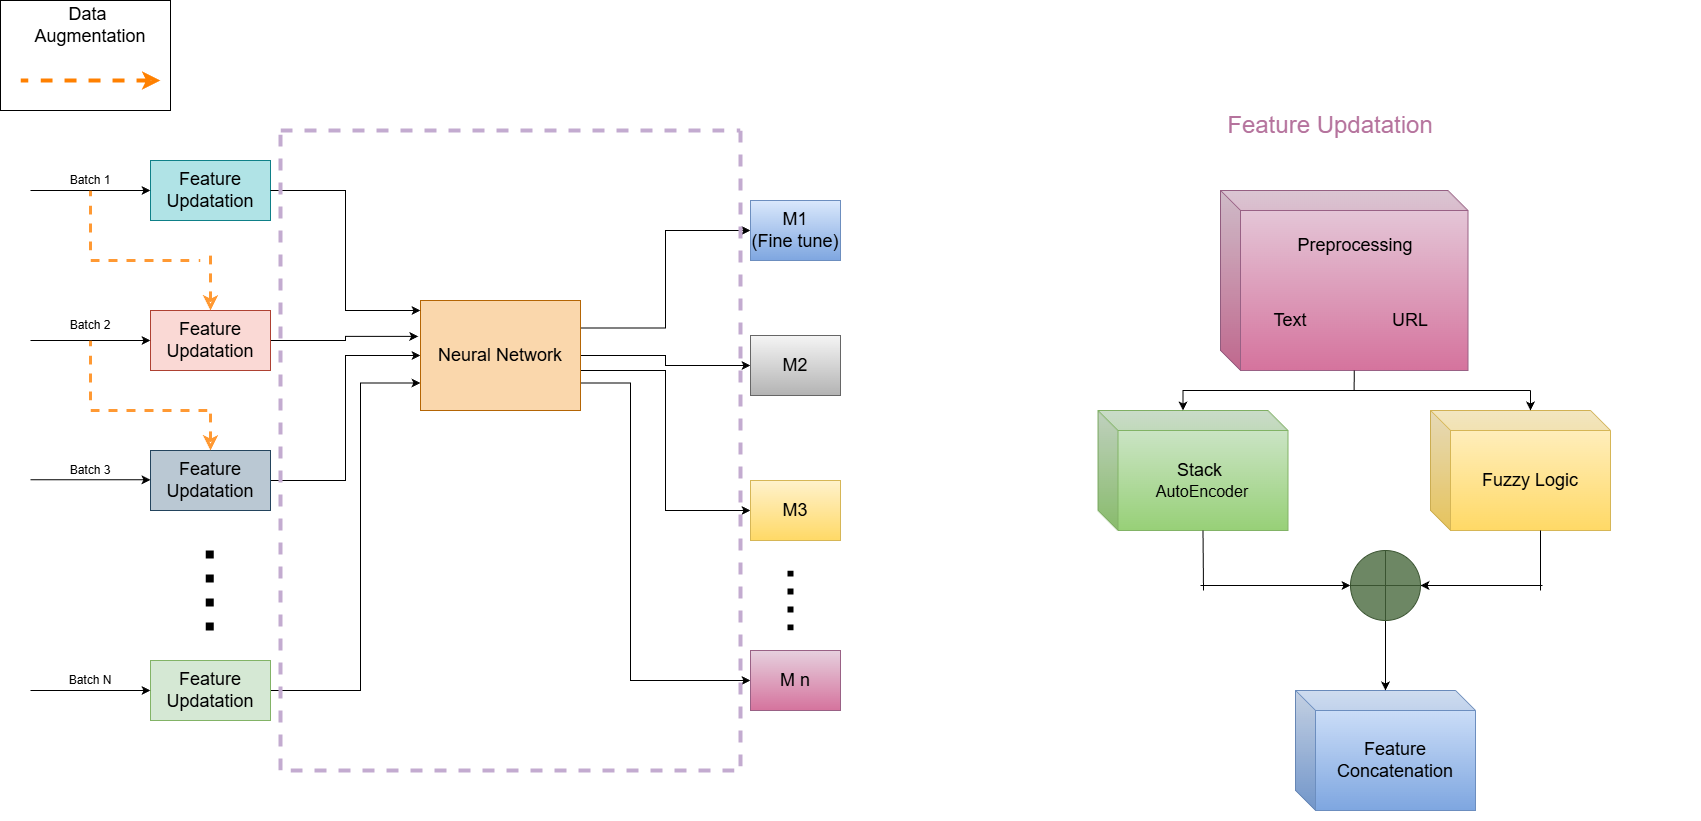
\includegraphics[width=\textwidth]{images/Review2_architecture.drawio.png}
\caption{Architecture Design of Proposed System}
\label{fig:architecture}
\end{figure}

In parallel to the process of updating features in batches, there is also a Data Augmentation module in the system that introduces diversity and variability to the training data. Whether it is the creation of new data samples synthetically or the creation of new samples from the existing ones, the data augmentation module is responsible for enhancing the generalization capability of the neural network as well as ensuring that it does not overfit. The process of updating features in batches and data augmentation ensures that the learning process remains stable even when the input batches have different distributions and structures.

On the right side of the architecture, the internal workflow of the Feature Updation Module has been shown in more detail. The Preprocessing module processes two types of data, Text and URL, thereby ensuring that both types of data are properly preprocessed. The preprocessed data is then fed to a Stacked Autoencoder, which reduces the dimensionality of the data and extracts meaningful latent features. Along with the autoencoder, a Fuzzy Logic module is used to process the uncertainties and linguistic nuances that are present in the data. The output of both the autoencoder and the fuzzy logic module is then combined using a Feature Concatenation module, resulting in a homogeneous feature vector that is then fed to the neural network for training and model development.

Overall, the architecture is designed to enable continuous learning, multi-modal feature refinement, and incremental model synthesis. By integrating preprocessing, fuzzy logic processing, stacked autoencoder-based feature extraction, and batch-based neural learning, the architecture provides a well-organized and scalable data pipeline from raw data to the final attack prediction.



\section{ELM Based Classification Architecture} 

The architecture of the system is designed to detect social engineering attacks by analyzing two different types of input data, which are text and URL features, by combining them into a single feature space. The system begins with the Data Loading module, where the data set containing the two types of input data is loaded into the system. Once the data is loaded, it is divided into its respective components and then sent to the two preprocessing paths.

The Text Preprocessing module performs operations such as text cleaning, lemmatization, removal of noise, and transformation into numerical vector form using TF-IDF vectorization followed by Truncated SVD for dimensionality reduction. The URL Preprocessing module extracts structural and lexical characteristics from the raw URL strings — including URL length, dot count, slash count, HTTPS presence, and character-level n-gram TF-IDF features — normalizes the values, and prepares them for feature learning.

After preprocessing, each data modality is sent to its corresponding Stacked Autoencoder (SAE) component — SAE Text and SAE URL. These autoencoders reduce the dimensionality of the processed inputs and learn meaningful latent feature representations. Instead of manually selecting features, the stacked autoencoders automatically extract hidden patterns and compress the information while preserving the critical characteristics of each data type. The text autoencoder follows a 200 → 100 → 50 → 100 → 200 architecture, producing a 50-dimensional encoded text representation, while the URL autoencoder follows a 68 → 60 → 50 → 60 → 68 architecture, producing a 50-dimensional encoded URL representation. Both the autoencoders are trained only on the Day 1 data, and their weights are frozen for the rest of the days. This ensures that the feature space is stable throughout the learning process.

The encoded outputs are then combined in the Combined Feature module. The Combined Feature module utilizes feature-level combination by concatenating the two 50-dimensional latent outputs into a combined 100-dimensional feature vector from Pipeline 1. Simultaneously, the Fuzzy-PGFDG module from Pipeline 2 generates a second 24-dimensional feature vector that encompasses 19 manual text and URL features expanded with 5 fuzzy descriptors: Typicality, Density, Homogeneity, Outlier Score, and Fuzzy Entropy. The output from Pipeline 1 and Pipeline 2 is then concatenated to generate the final 124-dimensional combined feature vector that encompasses a broad spectrum of information from both deep autoencoder latent outputs and fuzzy interpretable features.

This combined 124-dimensional feature vector is then fed into the Extreme Learning Machine (ELM) classifier. The ELM is a single-hidden-layer feedforward neural network that trains much faster than backpropagation-based models. The weights and biases of the hidden layer of the ELM are randomly generated and then fixed, and the output weights are determined in a single step using the Moore-Penrose pseudoinverse.

Finally, the trained ELM predicts the attack type using the combined 124-dimensional feature input. The ELM classifies each input instance into one of five categories: Baiting, Legitimate, Phishing, Pretexting, or Whaling. The ELM model of the previous day is intentionally deleted after each update, and only the new ELM model is saved, which ensures that the memory usage remains bounded for all incremental days. In conclusion, the architecture provides a systematic and optimized workflow from data loading to attack prediction, which covers preprocessing, automatic deep feature extraction, fuzzy feature generation, feature fusion, and analytically derived incremental classification.

\section{MODULES}
The proposed system is designed using a modular approach, where each module is designed to serve a distinct and critical purpose in the entire process of social engineering attack detection. The proposed system deals with two different types of data: textual content and URL features. Therefore, the proposed system consists of distinct modules designed specifically to deal with each type of data in an effective manner. The process begins with the Data Loading module, which loads the dataset and organizes it in the required formats. This module ensures that all the data is organized in the required and separated into text and URL components so that the subsequent stages receive clean and well-organized inputs.

Once the data is loaded, it is then passed through the Preprocessing module, which is tasked with the responsibility of preparing the data for further processing. Since each modality has its own unique features, two preprocessing pipelines are used. The text preprocessing entails the cleaning, tokenization, and vectorization of the raw text data, which makes it possible to transform the raw text data into numerical form. The URL preprocessing entails the extraction of structural and lexical features that help in the identification of malicious link patterns.

The processed data is then passed on to the Stacked Autoencoder (SAE) module. The SAE module is a very important part of the process of extracting significant hidden features from each type of data. Rather than using feature engineering, which is a time-consuming process, autoencoders are used to automatically extract hidden patterns and reduce the high-dimensional input into a lower-dimensional space. Autoencoders are employed independently for text data as well as URL modalities, ensuring that each type of data is mapped to its features based on its structural properties.

The output of the two autoencoders is merged in the Combined Feature module, where the combination of features at the feature level is performed. This module combines the latent features of all the modalities into a single feature representation. By combining the information from the text, URL data, the system obtains a better understanding of the samples, which helps in accurately identifying the attack patterns. The combined feature vector is the final input to the classification models.

The Classification module consists of one neural network model: Extreme Learning Machine (ELM). That model use the fused feature vector to predict the attack type. ELM uses randomly generated hidden nodes to train quickly.Model can be used to distinguish benign data from different types of social engineering attacks.

Finally, the Output module relays the result of the prediction to the user by specifying the attack category that has been identified. The modular structure of the system from data loading to preprocessing, feature learning, feature fusion, classification, and finally to output ensures that the system is efficient and scalable enough to handle multi-modal inputs for attack detection.

\subsection{Data Loading}
The Data Loading process is the backbone of the entire detection system because it is responsible for the importation, organization, and proper structuring of all the data used in the entire process. In this project, the data consists of two forms of information: text information and URL-related information. Because both forms of information have different properties, the Data Loading module is responsible for ensuring that both forms of information are properly identified and separated for the next modules to handle them in the correct manner.

When the data set is received, it starts with the process of reading the input from its source, such as CSV files, and validating the integrity of the data. It makes sure that there are no missing fields, that the data types are not incorrect, and that the formatting is consistent. The process also validates the number of samples, the alignment of the labels with the features, and breaks down the content into two structured parts. The text fields are stored in a separate structure so that they can be further preprocessed linguistically. The URL strings are stored in a separate area, awaiting URL-specific type extraction and cleaning.

Another significant task related to this step is the handling of errors and anomalies that are present in the raw data. These can be in the form of blank entries, incorrect entries, noisy symbols, or broken lines. The Data Loading is tasked with the preliminary filtering of the data to remove or point out erroneous data. In some cases, it is also tasked with documenting any discrepancies for later review, as a way of promoting transparency and debugging.

By the time the data loading process is completed, the system will have a well-structured format of text and URL, data. This is an important aspect because it will ensure that all the preprocessing modules receive the data in the exact format that they require.The Data Loading process is important because it will ensure the stability, reliability, and correctness of all the input data.

\subsection{Preprocessing Module}
The Preprocessing Module is a crucial component of the proposed system, as it attempts to transform the raw and unstructured inputs into clean, meaningful, and machine-readable formats. Considering the fact that the dataset comprises two distinct types of data: text and URL attributes, the preprocessing module comprises two distinct preprocessing pipelines. The two preprocessing pipelines are designed in such a manner that they are capable of handling the nature of their respective data modalities. The preprocessing module ensures that noise is eliminated, inconsistencies are resolved, and all data formats are transformed into structured formats that are ready for processing and feature extraction. The preprocessing module will ultimately be responsible for preparing the data for the Stacked Autoencoder and neural classification models.

\subsubsection{Text Preprocessing}

The Text Preprocessing is concerned with the cleaning and normalization of the text data acquired from posts, messages, or descriptions available on social media platforms. The raw text data usually comprises unnecessary characters, emojis, URLs, repeated symbols, case variations, and unnecessary stopwords that do not add any value to the meaningful information. This module is responsible for the cleaning of the text data by eliminating all the unnecessary characters and normalizing the text. The process starts with the conversion of text to lowercase to ensure consistency, followed by the removal of special characters, punctuation, and unnecessary spaces. The tokenization process is then used to split the sentences into individual words or meaningful pieces. Stemming or lemmatization is used to convert words to their root form to eliminate redundancy in the vocabulary.

After the cleaning process is finished, the text data must be converted into a form of numbers that can be handled by machine learning algorithms. A technique commonly employed for this task is {TF-IDF (Term Frequency-Inverse Document Frequency)}, which gives more significant to important words and reduces the effect of frequently occurring words. The TF-IDF value of a word $t$ in a document $d$ is given by the following formula:

\begin{equation}
\label{Eq1}
\text{TF-IDF}(t, d) = \text{TF}(t, d) \times \log\left( \frac{N}{\text{DF}(t)} \right)
\end{equation}


where,
\begin{itemize}
    \item $\text{TF}(t,d)$ is the frequency of term $t$ in document $d$,
    \item $N$ is the total number of documents, and
    \item $\text{DF}(t)$ is the number of documents containing term $t$.
\end{itemize}

This formula gives higher importance to terms that are frequent in one document but rare across others. In the context of attack detection, TF--IDF helps highlight contextual keywords and suspicious linguistic patterns often found in phishing, impersonation, or malicious messages.

However, TF--IDF vectors are often very high-dimensional, which can slow down the learning process and reduce model efficiency. To reduce dimensionality while preserving the essential meaning of the text,{Singular Value Decomposition (SVD)} is applied to the TF--IDF matrix. Mathematically, the decomposition is expressed as:

\begin{equation}
\label{Eq1}
X_{\text{TF-IDF}} = U \Sigma V^{T}
\end{equation}


where,
\begin{itemize}
    \item $U$ captures document-level patterns,
    \item $\Sigma$ contains the most important ``strengths'' or weights of the patterns, and
    \item $V^{T}$ represents word-level relationships.
\end{itemize}

That is, SVD helps in reducing the TF-IDF matrix, which is quite large, to its most significant components, so that the system can focus on the most significant linguistic aspects while ignoring the rest.

By carrying out the above-mentioned steps of cleaning, normalization, number conversion, and dimensionality reduction. The Text Preprocessing module ensures that only the most significant and compact representation of the text features are passed on to the feature extraction stage.

\subsubsection{URL Preprocessing}
The URL Preprocessing is intended to identify valuable structural and lexical patterns from the links of websites. URLs are known to hold important features of malicious activities, since attackers tend to incorporate deceptive components to deceive users. To identify these features, the preprocessing process tends to evaluate various components of each URL, including domain names, subdomains, path formats, query strings, and encoded characters. Features such as URL length, the number of numeric characters, the number of special characters, the presence of deceptive keywords, the use of HTTPS, or the presence of IP domain names are extracted and analyzed. Other lexical features might include character frequency patterns or entropy values. 

After feature extraction, the values of these features are normalized to maintain numerical consistency for all samples. This is done to make the machine learning model consider all features equally. The normalization process is carried out using the Standard Scaler as follows:

\begin{equation}
X_{\text{norm}} = \frac{X - \mu}{\sigma}
\end{equation}

where \(X\) is the original feature value, \(\mu\) is the mean of the feature across all samples, and \(\sigma\) is the standard deviation. This transformation ensures that features with larger numerical ranges do not dominate those with smaller ranges, improving model performance and stability.

The resulting cleaned and structured URL features help the system distinguish between normal links and deceptive or malicious URLs, significantly contributing to accurate attack detection.


\subsection{Stacked Autoencoder (SAE) Module}
The Stacked Autoencoder (SAE) module is given the task of extracting hidden patterns from the preprocessed data and then reducing the dimensionality of the data while preserving the crucial information. Since the system handles two different types of inputs, namely text and URL, two different autoencoders are used: SAE Text and SAE URL. Both autoencoders are trained separately to extract the important hidden patterns based on their respective data types.

\subsubsection{SAE Text Module}
The purpose of the SAE Text module is to reveal the hidden patterns in the linguistic and semantic structures from the preprocessed text data. The text data is expected to have complex patterns, word relations, and hidden semantic information that are difficult to model using simple and manually designed features. The SAE Text module automatically discovers the patterns by compressing the input text using multiple layers, creating a latent space that captures the essential characteristics of the text.

In the encoding process, the input text is compressed step by step, and each layer learns to capture the essential relations among words, phrases, or context-dependent features. To introduce non-linearity and allow the network to model complex relations, {LeakyReLU activation} is used in the hidden layers. The LeakyReLU activation function is defined as:

\begin{equation}
\text{LeakyReLU}(x) =
\begin{cases} 
x, & \text{if } x > 0 \\
\alpha x, & \text{if } x \le 0
\end{cases}
\end{equation}

where \(\alpha = 0.2\). This activation allows small negative values to pass through instead of setting them to zero, preventing neurons from becoming inactive and helping the network learn more robust representations.

The encoding process results in a compact vector representation that encodes the semantic essence of the text. The decoding process is tasked with the responsibility of recovering the original input from the latent vector, ensuring that the compressed vector is semantically meaningful. Although the reconstructed text is not used in the system, this process ensures that the latent vector preserves the most important aspects of the text.

SAE Text reduces noise and redundancy by converting raw text into dense vectors, hence reducing the dimensionality of the input data. The representation form of the input data is of high quality and is an ideal input for the classifiers, which can easily classify the malicious content. SAE Text automates the feature extraction process of the input text data.


\subsubsection{SAE URL Module}
The SAE URL module is concerned with learning structural and behavioral patterns from URL data. URLs are known to have indicators of potential attacks, including suspicious subdomains, path patterns, query strings, and encoded characters. The SAE URL module is able to learn these patterns by compressing the URL features into latent vectors.

During the encoding process, the module gradually decreases the dimensionality of the URL features, learning the relationships between structural elements, character distributions, and other lexical features. The latent vector learned from this process captures the behavior of the URL, making it easier for classifiers to distinguish between malicious and benign behavior. During the decoding process, the input URL is reconstructed to ensure that the key information is captured in the compressed form.

The SAE URL module removes unnecessary information, focusing only on the information that is crucial in making a distinction between normal and malicious URLs. The SAE URL module enhances the performance of the MLP and ELM classifiers by producing high-quality compact vectors. This module ensures that the system is able to process a large amount of URL information while still being accurate in attack detection.

\subsection{Combined Feature Module}
The Combined Feature module is a feature-level fusion module where the latent features extracted from the two Stacked Autoencoders are combined. Once each modality, text, and URL, has been represented as a compact feature vector, the vectors are combined to represent the input instance. This is an important step in the process as it enables the system to process both types of input simultaneously, thus enhancing its capability to identify complex attack patterns.

The concatenation of the latent vectors can be represented as:

\begin{equation}
X_{\text{fused}} = X_{\text{bottleneck}}^{\text{text}} \; \| \; X_{\text{bottleneck}}^{\text{url}} \; \| \; 
\end{equation}

where \(X_{\text{bottleneck}}^{\text{text}}\)and \(X_{\text{bottleneck}}^{\text{url}}\)are the latent vectors obtained from the SAE Text, SAE URL, and SAE Tabular modules, respectively. The symbol \(\|\) denotes vector concatenation. This step simply concatenates the three vectors together, forming a single unified feature vector that aggregates information from all three modalities. In doing so, the classifier is provided with a more informative representation of each sample, one that aggregates individual and cross-modal patterns.

The module also maintains structural consistency of the aggregated vector for all samples by addressing feature alignment, dimension consistency, and order. This structured unified representation serves as the input to the neural classifiers, allowing them to make more informed decisions. For instance, a phishing attack may contain suspicious text features, irregular URL features, and irregular metadata features; when all three modalities are aggregated, the system is able to identify these patterns more effectively.

The Combined Feature module consolidates multi-modal latent features into a single structured vector, enhancing the system’s predictive power and supporting precise attack classification.

\subsection{Fuzzy Feature Generation}

To increase class discrimination and model uncertainty in the detection of social engineering attacks, a Probabilistic Gaussian Fuzzy Distribution Generator (PGFDG) is employed in the fuzzy feature extraction framework. The primary aim of this component is to convert the normalized manual features into fuzzy features that are uncertainty-aware.

As Shown in ~\ref{fig:Fuzzy}, firstly, 19 manual features (11 text features and 8 URL features) are extracted and normalized using StandardScaler to ensure stable statistical calculations. The normalized features are then processed class-wise to generate fuzzy features for each attack class.

For each class, statistical parameters such as mean, standard deviation, and median are computed. Based on these, different fuzzy attributes are derived. {Typicality} is derived using a Gaussian membership function to measure the degree of membership of the sample to the class. {Core Membership} and {Boundary Proximity} measure the centrality and boundary samples for the cluster. {Density Score} measures the local density of the samples, while {Centrality} and {Compactness} measure the structural contribution of the class.

\begin{figure}[H]
    \centering
    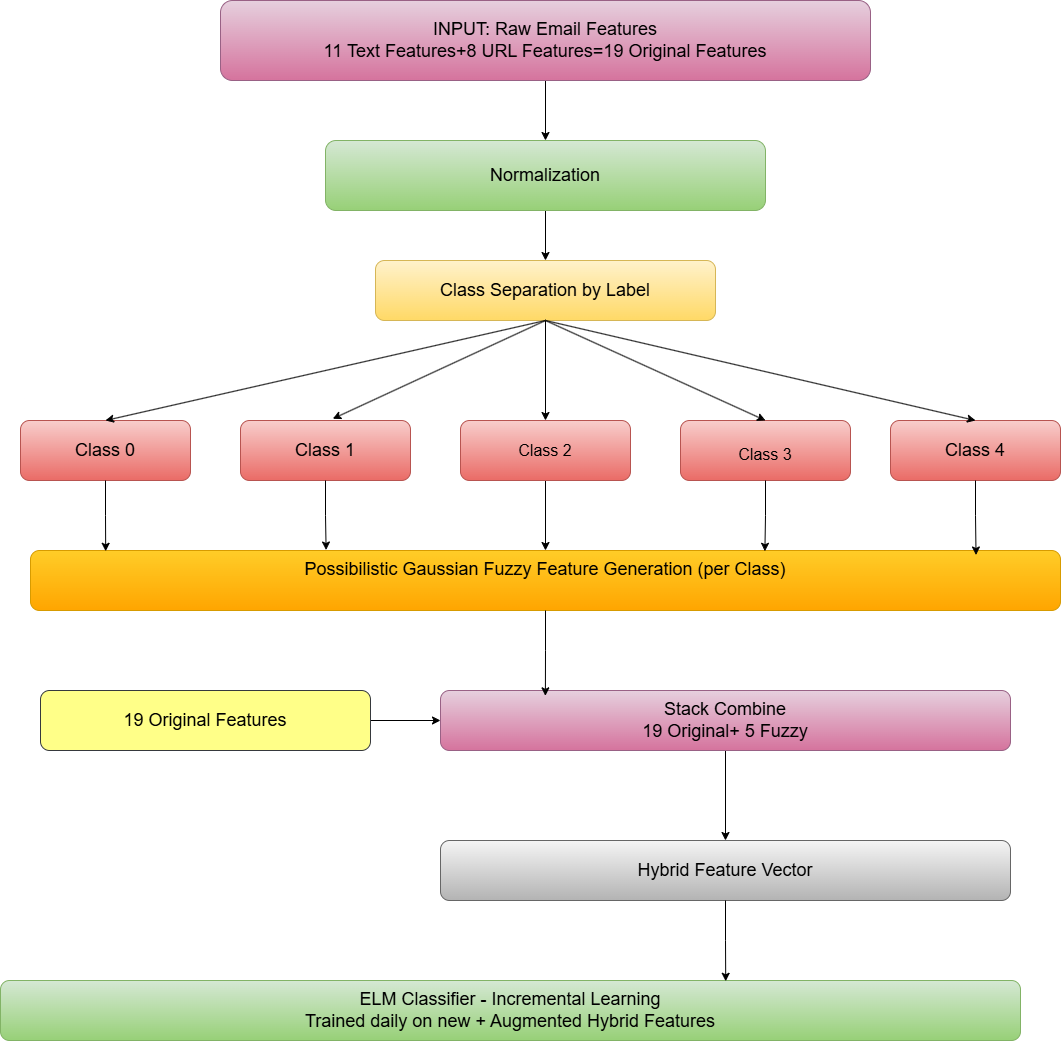
\includegraphics[width=\textwidth]{images/workflow_diagram.png}
    \caption{PGFDG-Based Feature Extraction}
    \label{fig:Fuzzy}
\end{figure}

Other features are: {Subspace Memberships} (computed on feature subsets), {Homogeneity}(relationship with class mean), {Outlier Score} (computed using modified Z-score and median absolute deviation), {Stability} (distance to median), and {Fuzzy Entropy}.

Among the 16 fuzzy features, five most representative features—Typicality, Density Score, Homogeneity, Outlier Score, and Fuzzy Entropy—are selected and incorporated into the normalized manual features.

A correction is applied to ensure that the fuzzy features are stored in the correct order using boolean masking.

The PGFDG-based fuzzy modeling approach improves robustness by incorporating uncertainty, structural density, and anomalies to improve class separation and generalization capabilities in the incremental social engineering attack detection problem.The detailed procedure for generating the fuzzy descriptors is presented in Algorithm~\ref{alg:fuzzy_pgfdg}.\\

\begin{algorithm}
\caption{Fuzzy Probability-Guided Feature Descriptor Generator (Fuzzy-PGFDG)}
\label{alg:fuzzy_pgfdg}
\begin{algorithmic}[1]

\Require $X \in \mathbb{R}^{n \times 19}$, 
$y \in \mathbb{R}^{n}$, 
$k=5$, $\epsilon=10^{-6}$

\Ensure $H \in \mathbb{R}^{n \times 24}$

\State $\hat{X} \gets (X - \mu_X)/\sigma_X$

\For{each class $c \in \{1,\dots,C\}$}

    \State $X_c \gets \{\hat{x}_i : y_i=c\}$

    \State $\mu_c \gets \frac{1}{|X_c|} \sum \hat{x}_i$

    \State $\Sigma_c \gets
    \frac{1}{|X_c|-1}
    \sum (\hat{x}_i-\mu_c)(\hat{x}_i-\mu_c)^T
    + \epsilon I$

    \State $M_c \gets \text{median}(X_c)$
    \State $\text{MAD}_c \gets \text{median}(|\hat{x}_i-M_c|)$

    \State $r_c \gets
    \text{percentile}_{25}
    (\|\hat{x}_i-\mu_c\|_2)$

\EndFor

\For{each sample $\hat{x}_i$}

    \State $d_M \gets
    \sqrt{(\hat{x}_i-\mu_c)^T
    \Sigma_c^{-1}
    (\hat{x}_i-\mu_c)}$

    \State $T_c \gets
    \exp\!\left(-\frac{1}{2} d_M^2\right)$

    \State $D_c \gets
    \frac{
    |\{x_j \in X_c :
    \|x_j-\hat{x}_i\|_2 \le r_c\}|
    }{|X_c|}$

    \State $\mathcal{H}_c \gets
    \frac{\hat{x}_i \cdot \mu_c}
    {\|\hat{x}_i\|_2 \|\mu_c\|_2}$

    \State $O_c \gets
    \min\!\left(
    1.0,
    \frac{0.6745\|\hat{x}_i-M_c\|_2}
    {\|\text{MAD}_c\|_2+\epsilon}
    \right)$

    \State $t \gets T_c$
    \State $\bar{t} \gets 1-t$

    \State $E_c \gets
    -t\log_2(t+\epsilon)
    -\bar{t}\log_2(\bar{t}+\epsilon)$

    \State $\phi_i \gets
    [T_{y_i},D_{y_i},
    \mathcal{H}_{y_i},
    O_{y_i},E_{y_i}]$

\EndFor

\State $F \gets [\phi_1|\dots|\phi_n]^T$

\State Select top $k$ least-correlated fuzzy features

\State $H \gets [\hat{X}\;|\;F_{\mathcal{S}}]$

\State \Return $H$

\end{algorithmic}
\end{algorithm}

\FloatBarrier
\subsection{Data Augmentation}

For the purpose of reducing the effects of class imbalance and catastrophic forgetting in the incremental learning framework, a supervised DAIL (Deterministic Alternating Interleaving Logic) data augmentation approach is proposed. The proposed approach uses the learned clusters of previous tasks to favor past class patterns when new data samples arrive.

As shown in ~\ref{fig:Data_aug}, the augmentation procedure is dependent on the hybrid features derived from the previous training phases. The data points are categorized based on their cluster labels, and for each category, the major class label is determined. The number of data points to be generated for the augmentation procedure is regulated by an augmentation ratio parameter $\alpha$, which determines the ratio of the augmentation procedure to the number of new data points entering the system. The number of augmentations is limited to enable proper pairing.

The synthetic instances are created through an alternating interleaving mechanism of features. Two parent instances are randomly chosen from the same cluster. The synthetic instances are created through an alternating fashion of choosing feature values from the two parent instances, where even-indexed features are chosen from one parent instance and odd-indexed features are chosen from the other parent instance, and then switched for the second synthetic instance. This deterministic interleaving process ensures that the characteristics of the class are maintained while new combinations of feature patterns are created. Since both parent instances belong to the same cluster, the labels are maintained.

\begin{figure}[H]
    \centering
    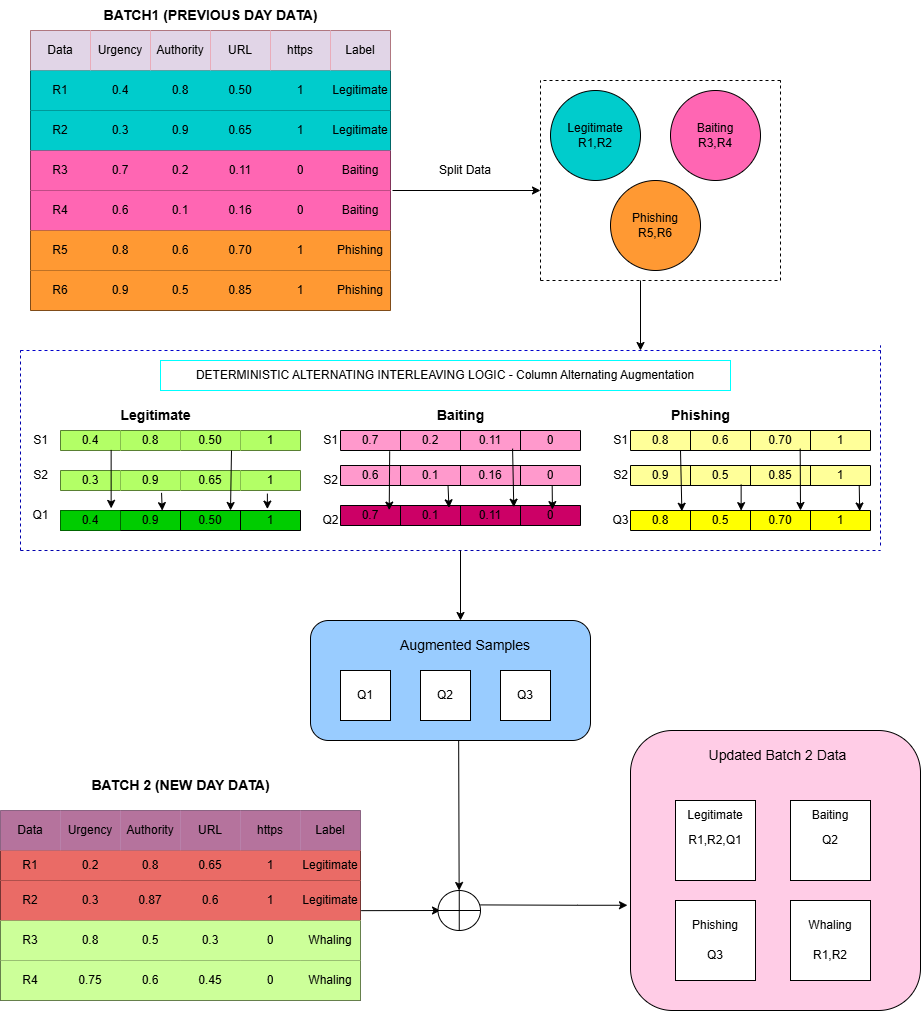
\includegraphics[width=\textwidth]{images/FYP_Augmentation.png}
    \caption{Data Augmentation- Column Alternating Approach}
    \label{fig:Data_aug}
\end{figure}

Each synthesized example is then labeled with the strongest class label from its source cluster, and the cluster labels are kept. The method obtains the expanded feature matrix, class labels, cluster labels, and a summary of the number of synthesized examples per class.

In conclusion, the DAIL method is a simple and supervised augmentation technique for controlled synthetic data generation. The method assists in preserving class distributions from previous learning without storing the whole past data, thus facilitating stable incremental learning and improving model robustness for dynamic social engineering attack detection.The detailed procedure of the DAIL augmentation process is presented in Algorithm~\ref{alg:dail}.

\begin{algorithm}[H]
\caption{DAIL Column-Alternating Augmentation}
\label{alg:dail}
\begin{algorithmic}

\Require 
$S^{(d-1)} \in \mathbb{R}^{m \times 124}$, 
$y^{(d-1)} \in \mathbb{R}^{m}$, 
$\mathrm{CID}^{(d-1)} \in \mathbb{R}^{m}$, 
$X_{\text{new}}^{(d)} \in \mathbb{R}^{p \times 124}$, 
$\alpha$, $K$

\Ensure 
$X_{\text{total}}^{(d)} \in \mathbb{R}^{(p+q)\times124}$, 
$y_{\text{total}}^{(d)} \in \mathbb{R}^{p+q}$

\State \textbf{Phase 1: Per-Cluster Augmentation Budget}

\State $n_{\text{budget}} \gets \alpha \cdot p$

\For{$k = 1$ to $K$}
    \State $S_k \gets \{ s_i \in S^{(d-1)} : \mathrm{CID}_i = k \}$
    \State $n_k \gets |S_k|$
    \State $n_k^{\text{aug}} \gets 
    \min\!\left(\left\lfloor\frac{n_k}{2}\right\rfloor,
    \left\lfloor\frac{n_{\text{budget}}}{K}\right\rfloor\right)$
    \State $n_k^{\text{aug}} \gets n_k^{\text{aug}} - 
    (n_k^{\text{aug}} \bmod 2)$
\EndFor

\Statex
\State \textbf{Phase 2: Column-Alternating Generation}

\State $X_{\text{aug}} \gets \emptyset$, 
$y_{\text{aug}} \gets \emptyset$

\For{$k = 1$ to $K$}

    \State $\{ s_1, s_2, \dots, s_{n_k^{\text{aug}}} \} 
    \gets$ random samples from $S_k$ (without replacement)

    \For{$i = 1,3,5,\dots,n_k^{\text{aug}}-1$}

        \For{$j = 0$ to $123$}

        \[
        Q_1[j] =
        \begin{cases}
        s_i[j] & \text{if } j \bmod 2 = 0 \\
        s_{i+1}[j] & \text{if } j \bmod 2 = 1
        \end{cases}
        \]

        \[
        Q_2[j] =
        \begin{cases}
        s_{i+1}[j] & \text{if } j \bmod 2 = 0 \\
        s_i[j] & \text{if } j \bmod 2 = 1
        \end{cases}
        \]

        \EndFor

        \State $y_{Q_1} = y_{Q_2} \gets 
        \mathrm{mode}(\{ y_i : \mathrm{CID}_i = k \})$

        \State $X_{\text{aug}} \gets 
        X_{\text{aug}} \cup \{Q_1, Q_2\}$

        \State $y_{\text{aug}} \gets 
        y_{\text{aug}} \cup \{y_{Q_1}, y_{Q_2}\}$

    \EndFor
\EndFor

\Statex
\State \textbf{Phase 3: Merge}

\State $X_{\text{total}}^{(d)} \gets 
\begin{bmatrix}
X_{\text{new}}^{(d)} \\
X_{\text{aug}}
\end{bmatrix}$

\State $y_{\text{total}}^{(d)} \gets 
\begin{bmatrix}
y_{\text{new}}^{(d)} \\
y_{\text{aug}}
\end{bmatrix}$

\Statex
\State \textbf{Phase 4: Memory Cleanup}

\State Delete $S^{(d-1)}$, Delete $\mathrm{ELM}^{(d-1)}$
\State $S^{(d)} \gets X_{\text{total}}^{(d)}$

\State \Return $X_{\text{total}}^{(d)}, y_{\text{total}}^{(d)}$

\end{algorithmic}
\end{algorithm}


\subsection{ELM Classifier}

The Extreme Learning Machine (ELM) classifier provides an extremely efficient method for training a neural network classifier compared to the standard training method. Unlike the MLP classifier, which needs to be trained using the backpropagation method, the ELM classifier initializes the weights and biases of the hidden layers randomly and keeps them fixed throughout the entire training process. This reduces the computational overhead involved in training a neural network classifier. Once the transformation of the hidden layers is determined, the ELM classifier computes the output weights in one step, allowing for extremely fast training.

Given an input matrix \(X \in \mathbb{R}^{N \times 150}\) and the corresponding output label matrix \(Y \in \mathbb{R}^{N \times K}\), the hidden layer output of ELM is computed as

\begin{equation}
H = \sigma\!\left(\mathbf{1}\beta_0 + XW\right)
\end{equation}

where \(W \in \mathbb{R}^{150 \times L}\) is a randomly initialized weight matrix, \(\beta_0 \in \mathbb{R}^{1 \times L}\) is a random bias row vector, \(L\) is the number of hidden neurons (here \(L=150\)), and \(\mathbf{1}\in\mathbb{R}^{N\times 1}\) is a column vector of ones used to broadcast the bias across \(N\) rows. The activation \(\sigma\) is the sigmoid function:

\begin{equation}
\sigma(x) = \frac{1}{1 + e^{-x}}
\end{equation}


This activation function projects the actual inputs to the range \((0,1)\), which helps the hidden layer to produce a smooth non-linear projection of the fused features. Since \(W\) and \(\beta_0\) are random variables and are fixed, the hidden layer can be treated as a feature projector that projects the input into an informative representation very quickly.

Once the hidden layer output matrix \(H\in\mathbb{R}^{N\times L}\) is obtained, the output weights \(\beta\in\mathbb{R}^{L\times K}\) are computed analytically using the Moore–Penrose pseudoinverse:

\begin{equation}
\beta = H^{\dagger}Y
\end{equation}

with one common expression for the pseudoinverse (when \(H^{T}H\) is invertible) given by

\begin{equation}
H^{\dagger} = (H^{T}H)^{-1}H^{T}
\end{equation}


This provides the least squares solution that directly relates the features of the hidden layers to the desired outputs in a single linear solve. However, in practice, to improve numerical stability, especially when \(H^{T}H\) is close to being singular, a regularized solution is usually used:

\begin{equation}
\beta = \left(H^{T}H + \lambda I\right)^{-1} H^{T} Y
\end{equation}

where \(\lambda>0\) is a small regularization parameter and \(I\) is the \(L\times L\) identity matrix.

With the application of this analytical training method, the ELM classifier is able to efficiently learn the decision boundaries based on the combined latent features obtained from the Stacked Autoencoders. This is particularly useful in scenarios that require rapid model training or system update. The complementary nature of the ELM classifier with the MLP classifier further enhances the robustness of the system, which is capable of rapid and precise identification of various patterns of social engineering attacks.

As shown in Algorithm~\ref{alg:ELM}, the Extreme Learning Machine computes the hidden layer outputs and the output weights analytically.


\begin{algorithm}[H]
\caption{Algorithm for Extreme Learning Machine (ELM)}
\label{alg:ELM}
\begin{algorithmic}[1]


\State \textbf{Input:} Training feature matrix $X$, label vector $Y$, number of hidden neurons $N_h$, activation function

\State Randomly initialize hidden layer weights $W_h$ and biases $b_h$

\State Compute hidden layer output matrix $H$:
\For{each sample $x_i$ in $X$}
    \State $h_i = activation(W_h \cdot x_i + b_h)$
\EndFor

\State Compute output weights $\beta$ using Moore--Penrose pseudoinverse:
\State $\beta = pinv(H) \cdot Y$

\State \textbf{Training complete:} ELM model is ready after obtaining $\beta$

\State \textbf{Prediction:} For a new sample $x_{\text{new}}$:
\State $h_{\text{new}} = activation(W_h \cdot x_{\text{new}} + b_h)$
\State Output label prediction: $y_{\text{new}} = h_{\text{new}} \cdot \beta$

\end{algorithmic}
\end{algorithm}
\subsection{Incremental Learning}

The proposed system uses a structured four-day incremental learning method to simulate the occurrence of social engineering attack types in the real world. Instead of training a single model, the classifier is updated as new classes and samples are added. This method enables the system to adapt continuously without catastrophic forgetting.

On Day 1, the training of the model is performed on the first three classes: Legitimate, Phishing, and Baiting. A fixed number of samples for each class are selected to form the initial training set. The hybrid feature extraction is performed by the stacked autoencoder (Pipeline 1) and fuzzy PGFDG features (Pipeline 2), resulting in a 124-dimensional feature space. The dataset is split using an 80/20 stratified train-test split, and an Extreme Learning Machine (ELM) classifier is trained. The number of hidden neurons is dynamically adjusted as $200 \times n_{\text{classes}}$, which is adjusted based on the number of classes.

On Day 2, new samples are added from selected classes. Instead of retraining the model from scratch, the approach includes supervised DAIL augmentation using the stored Day 1 features. New samples are created cluster-wise and combined with the new incoming samples. The pool of samples is then divided and used to train a new ELM model. After the successful training of the model, the old model instance is deleted to save memory.

On Day 3, a new class (Pretexting) is introduced, thus adding to the number of classes in the classification task. Once again, the same procedure is followed: new data is passed through frozen encoders from Day 1 to maintain consistency in the feature space, DAIL augmentation is performed based on the representations from Day 2, and a new ELM is learned. The size of the hidden layer is automatically determined based on the new number of classes.

On Day 4, all five classes (Legitimate, Phishing, Baiting, Whaling, and Pretexting) are trained together. New data is combined with the learned features from Day 3, and a new ELM is trained. Confusion matrix and test accuracy are computed to check the performance. In all stages, the feature encoders are frozen after Day 1 to ensure a fixed feature space.

This incremental learning approach has several advantages. Firstly, it is possible to incrementally add new attack types without the need to retrain on the whole past data. Secondly, the supervised DAIL learning approach assists in reinforcing past class distributions learned by the model, hence combating catastrophic forgetting. Thirdly, the dynamic scaling of hidden neurons assists the ELM classifier in adapting to the increasing complexity of the classes. Finally, past model copies are deleted after each update, hence promoting efficient memory use.

The incremental learning approach hence assists in adaptive, scalable, and memory-efficient social engineering attack detection.
 % DESIGN
% Chapter 3

\chapter{EXPERIMENTAL RESULTS AND PERFORMANCE ANALYSIS}

\section{DATASET DESCRIPTION}
In order to avoid the classifier being biased towards the majority classes, it includes a well-balanced and multi-modal dataset with 2,500 samples that are evenly distributed among the five categories of social engineering attacks, with around 500 samples each category, as demonstrated in in~\ref{tab:dataset}.
\begin{table}[h!]
\centering
\caption{Dataset Description}
\label{tab:dataset}
\footnotesize
\renewcommand{\arraystretch}{1.05}
\setlength{\tabcolsep}{3pt}

\resizebox{\textwidth}{!}{%
\begin{tabular}{|p{2.5cm}|p{2cm}|p{9cm}|}
\hline
\textbf{Attack Category} & \textbf{Number of Samples} & \textbf{Description} \\ \hline

Phishing  & 496 & Fraudulent messages aiming to steal sensitive information. \\ \hline
Whaling   & 500 & High-profile targeting attacks aimed at executives. \\ \hline
Pretexting & 518 & Social manipulation using fabricated scenarios to extract data. \\ \hline
Baiting   & 485 & Luring users using fake offers or malicious links. \\ \hline
Legitimate & 501 & Non-malicious samples used as control/normal data. \\ \hline

\textbf{Total} & \textbf{2500} & Balanced dataset across all five classes. \\ \hline

\end{tabular}
}
\end{table}


%
\subsection{Dataset Composition} 
\begin{itemize}
    \item Phishing Attacks: 496 examples of widespread, fraudulent emails that target private information and login passwords.
    \item Whaling Attacks: 500 examples of targeted emails sent to high-value employees and executives.
    \item Pretexting Attacks: 518 instances of dishonest correspondence creating fictitious connections or authority.
    \item Baiting Attacks: 485 samples contain enticing communications with malicious attachments or links.
    \item Legitimate Communications: 501 examples of legitimate communications and real organizational data samples.
\end{itemize}
\subsection{Dataset Distribution} 
Baiting, legitimate, phishing, pretexting, and whaling are the five categories of social engineering attack types that make up the dataset's 2,500 labeled email examples. Each category has between 485 and 518 examples, guaranteeing a nearly balanced class distribution that prevents any one class from overshadowing the learning process. The dataset is separated into four days of incremental learning, in contrast to the usual static dividing of the train and test sets. This simulates a realistic real-world streaming scenario in which fresh data and attack classes are gradually introduced over time.

An 80:20 stratified split is applied separately to the whole pool of examples for each incremental learning day, which consists of both fresh real instances and DAIL-generated synthetic examples from the cluster storage from the day before. A bias toward majority classes in the assessment process is prevented by the stratified split, which guarantees that the class distribution in both the training and test sets appropriately reflects the distribution of active courses for that specific day. The daily distribution is as follows:

\begin{table*}[h]
\centering
\caption{Dataset Distribution}
\label{tab:dataset_distribution}
\resizebox{\textwidth}{!}{
\begin{tabular}{|c|c|c|c|c|c|c|}
\hline
\textbf{Day} & \textbf{Classes Active} & \textbf{New Samples} & \textbf{Augmented} & \textbf{Total Pool} & \textbf{Train (80\%)} & \textbf{Test (20\%)} \\ \hline
Day 1(baiting,phishing,legitimate) & 3 & 700 & 0   & 700  & 560 & 140 \\ \hline
Day 2(baiting,phishing,legitimate,whaling) & 4 & 450 & 180 & 630  & 504 & 126 \\ \hline
Day 3(baiting,phishing,legitimate,whaling,pretexting) & 5 & 576 & 220 & 796  & 636 & 160 \\ \hline
Day 4(baiting,phishing,legitimate,whaling,pretexting) & 5 & 775 & 348 & 1,123 & 898 & 225 \\ \hline
\textbf{Total} & -- & \textbf{2,501} & \textbf{748} & \textbf{3,249} & \textbf{2,598} & \textbf{651} \\ \hline
\end{tabular}
}
\end{table*}

The per-class sample composition on each day mentioned in ~\ref{tab:dataset_distribution}.  represents three different scenarios that the incremental system needs to deal with. In the first scenario, a class receives new real samples and new samples from previous days, which gives a strong training example. In the second scenario, a class receives no new real samples but receives DAIL-augmented samples, which is the most important scenario for preventing catastrophic forgetting, which happens on Day 2 for Baiting and Phishing and on Day 3 for Legitimate and Whaling. In the third scenario, a new class emerges for the first time with only real samples and no augmentation history, which happens on Day 2 for Whaling and on Day 3 for Pretexting.
\subsection{Feature Representation} 
Text Modality:Email body and subject line content transformed into 300-dimensional vectors by using TF-IDF weighting and subsequent matrix factorization.\\
URL Modality:URLs are extracted and represented as 68-dimensional feature vectors that encode syntactic characteristics, domain information, and structural patterns.\\
%BDDs – directed acyclic graph of Boolean expressions. If the variables occur in the same ordering on all paths from root to leaves, we call this OBDD.
%Example: $t=(x_1\&y_1)|(x_2\&y_2)$
%Shannon expansion of t in order x1,y1,x2,y2

%  $t            =x_1\to t_1,t_{01}$

%  $t_1        =y_1\to 1,t_{01}$

%  $t_{01}   =x_2\to t_{011},0$

%  $t_{011} =y_2\to 1,0$
\section{ECOSYSTEM}
\subsection{Hardware Configuration} 
Google Colab’s free-tier runtime provides the following hardware
configuration, which was used throughout model development:
\begin{itemize}
    \item \textbf{RAM:} 16 GB System memory 
    \item \textbf{Storage:}Google Drive integration for accessing datasets and saving model checkpoints.
    \item \textbf{Computational Device:} CPU-based processing.
    \item \textbf{Execution Environment:}Cloud-based runtime with automatic
session management
    
\end{itemize}

\subsection{Software Environment}
The entire system was developed using Python in the Google Colab
environment, supplemented with essential machine learning libraries. The main software components used :
\begin{itemize}
    \item \textbf{Programming Language:} Python 3.8.10

    \item \textbf{Machine Learning Libraries:} scikit-learn 1.1.3, NumPy 1.23.5, Pandas 1.5.3
    \item \textbf{Data Processing:} Scikit-learn preprocessing and feature scaling utilities.
    \item \textbf{Development Environment:} Jupyter Notebook on Google Colab (cloud-based, CPU instances)
\end{itemize}

\section{EXPERIMENTS CONDUCTED}
\subsection{Incremental Learning Scenario Design}
The data was divided into four sequential pieces, each representing four business days, in order to more closely resemble a real-world example of incremental learning, when social engineering attacks change over time and new attack classes appear gradually. A fresh collection of examples is provided every day, and starting on Day 3, new attack classes that weren't there in the days before start to appear. This is done specifically to assess the model's capacity to absorb new information while maintaining the knowledge acquired from earlier days—the stability-plasticity issue that the DAIL method resolves.

\textbf{Day 1 — Initial Training (3 Classes)}\\
Initially, 700 samples from three attack classes—250 legitimate, 250 phishing, and 200 baiting attacks—were used to set up the system. On this day, all of the TF-IDF, SVD, and scaler transformers are applied, and the Stacked Autoencoder is trained from scratch to create the foundation for the feature space. For the duration of the incremental learning period, the frozen transformers from Day 1 will be used on all subsequent days to keep the feature space constant. On Day 1, no augmentation is carried out because there is no prior history to draw from.

\textbf{Day 2 — First Incremental Update (4 Classes)}\\
The second batch introduces 450 new samples — 150 Legitimate and 300 Whaling. Notably, Phishing has zero new real arrivals on Day 2, creating the risk that the updated model will forget previously learned Phishing patterns. DAIL augmentation is applied with $\alpha$, generating some synthetic Phishing samples from Day 1's cluster,few augmented Baiting samples, and few augmented Legitimate samples — totalling augmented samples. These are merged with the new samples to form a sample total training pool.

\textbf{Day 3 — Second Incremental Update (5 Classes)}\\
Test accuracy dropped to 86.25\% following the introduction of Pretexting. Pretexting shares formal, authority-driven language features with both Legitimate and Whaling, causing inter-class confusion. Legitimate had zero new arrivals but was sustained through DAIL-augmented samples, demonstrating effective catastrophic forgetting prevention.

\textbf{Day4 -Third Incremental Update (5 Class)}\\
Test accuracy reached 83.56\% on 225 test samples with all five classes now active. The Day 4 total training pool comprised 1,123 samples — 775 new real samples combined with 348 DAIL-augmented samples drawn from the Day 3 cluster storage. This is the largest training pool across all four days, reflecting the cumulative growth of the incremental system.The day wise data configuration is clearly mentioned in ~\ref{tab:day_wise_config}.

\begin{table}[h]
\centering
\caption{Day wise data configuration}
\label{tab:day_wise_config}
\resizebox{\textwidth}{!}{
\begin{tabular}{|c|c|c|c|c|c|c|c|c|}
\hline
\textbf{Day} & \textbf{New Samples} & \textbf{Classes Active} & \textbf{New Class Introduced} & $\alpha$ & \textbf{Augmented Samples} & \textbf{Total Pool} & \textbf{Train (80\%)} & \textbf{Test (20\%)} \\
\hline
Day 1(baiting,phishing,legitimate) & 700 & 3 & --- & --- & 0 & 700 & 560 & 140 \\
\hline
Day 2(baiting,phishing,legitimate,Whaling) & 450 & 4 & Whaling & 0.40 & 180 & 630 & 504 & 126 \\
\hline
Day 3(baiting,phishing,legitimate,Whaling,pretexting) & 575 & 4 & Pretexting & 0.50 & 220 & 796 & 636 & 160 \\
\hline
Day 4(baiting,phishing,legitimate,whailing,pretexting) & 775 & 5 & None & 0.60 & 348 & 1123 & 898 & 225 \\
\hline
\end{tabular}
}
\end{table}

\subsection{Stacked Autoencoder Experiment}
The first feature extraction was developed to produce deep and dense representations from the raw email text and URL features using a two-step approach: dimensionality reduction and autoencoder-based representation learning.

\textbf{Text Feature Extraction}\\ 
The body and subject of each email were concatenated and preprocessed using lemmatization and regex-based noise removal. A TF-IDF vectorizer with max vocabulary of 2,000 features and unigram-bigram range (1,2) was used to convert the preprocessed text into a sparse matrix. Truncated SVD with 200 components was used to reduce the sparse matrix to a dense 200-dimensional representation. A StandardScaler was used to normalize the output of SVD before passing it to the autoencoder.

The text autoencoder was designed with an architecture of 200$\rightarrow$100$\rightarrow$50$\rightarrow$100$\rightarrow$100$\rightarrow$200, employing \textit{Leaky ReLU} activation functions for all hidden layers and a linear activation for the output layer. The bottleneck layer provides a 50-dimensional encoded representation of the text. The model was trained using the Adam optimizer with Mean Squared Error (MSE) loss for 300 epochs and a batch size of 64.

\textbf{URL Feature Extraction}\\
Four URL characteristics --- URL length, number of dots, number of slashes, and presence of HTTPS --- were manually feature-engineered. In addition, a character-level TF--IDF vectorizer (\texttt{analyzer='char\_wb'}, \texttt{ngram\_range=(3,5)}, \texttt{max\_features=512}) was applied to the raw URL strings, followed by Truncated SVD with 64 components. These features were horizontally stacked to form a 68-dimensional URL feature matrix, which was normalized before training the autoencoder.

The URL autoencoder architecture was 68$\rightarrow$60$\rightarrow$50$\rightarrow$60$\rightarrow$68, again using \textit{LeakyReLU} activation functions, yielding a 50-dimensional encoded URL representation. The model was trained using the same configuration for 300 epochs.

\textbf{Frozen Feature Space}\\
One of the most important design choices is that the autoencoders and all the transformers (TF-IDF, SVD, and scalers) are trained only on Day 1 data, and their weights are set to be frozen for Days 2, 3, and 4. This guarantees that all 124-dimensional feature vectors for all four days are in the same feature space, allowing for a fair comparison and classification across all four days.

The two 50-dimensional outputs are concatenated to create the 100-dimensional output vector
\subsection{Fuzzy-PGDFG Experiment}
The second extracts interpretable, uncertainty-aware features using a fuzzy logic framework applied to manually engineered content features.

\textbf{Manual Feature Engineering}\\ 
Eleven text features are extracted per sample — urgency score, authority score, financial keyword score, credential keyword score, secrecy score, action score, routine score, length score, formality score, time pressure score, and grammar score. Eight URL features are extracted — URL presence, URL length ratio, dot count ratio, digit ratio, HTTPS flag, Shannon entropy, special character ratio, and subdomain count ratio. All 19 features are normalized using StandardScaler.

\textbf{Fuzzy Feature Generation}\\ 
For each class cluster, the Fuzzy-PGFDG computes 16 fuzzy descriptors per sample using Mahalanobis distance, neighborhood density estimation, subspace membership analysis, and entropy-based uncertainty quantification. From these 16, five diverse and non-redundant features are selected:

\begin{itemize}

\item \textbf{Typicality:} Computed as $\exp(-0.5 \times d_M^2)$ where $d_M$ is the Mahalanobis distance --- measures how representative the sample is of its class centroid.

\item \textbf{Density:} Local cluster compactness is encoded by the ratio of class neighbors within the 25th percentile radius.

\item \textbf{Homogeneity:}  Intra-class homogeneity is encoded by the Pearson correlation coefficient between the sample descriptor and class mean.

\item \textbf{Outlier Score:} a modified Z-score that uses the median absolute deviation to identify samples that are close to class borders.

\item \textbf{Fuzzy Entropy:} This measure encodes assignment uncertainty and is the normalized Shannon entropy of the typical/atypical membership pair.

\end{itemize}

2's final output, a 24-dimensional hybrid vector (19 manual + 5 fuzzy), is concatenated with 1's 100-dimensional output to create a 124-dimensional composite feature vector for classification.

\textbf{Data Augmentation Experiment}\\
The DAIL column-alternating augmentation was applied at the start of Days~2, 3, and~4 using the previous day's stored combined 124-dimensional feature matrix as the source pool. For each class cluster, pairs of samples are randomly selected without replacement, and two synthetic samples are generated per pair by alternating feature column values between the two parent samples:

\[
Q_1[j] =
\begin{cases}
S_1[j] & \text{if } j \bmod 2 = 0 \\
S_2[j] & \text{if } j \bmod 2 = 1
\end{cases}
\qquad
Q_2[j] =
\begin{cases}
S_2[j] & \text{if } j \bmod 2 = 0 \\
S_1[j] & \text{if } j \bmod 2 = 1
\end{cases}
\]

This guarantees that all generated samples remain within their parent cluster's feature distribution.The per-class augmentation outcomes across the three augmented days are mentioned in Table ~\ref{tab:per-class-aug}

\begin{table}[h]
\centering
\caption{Per-class augmentation outcomes}
\label{tab:per-class-aug}
\begin{tabular}{|c|c|c|c|p{4.5cm}|}
\hline
\textbf{Day} & \textbf{Class} & \textbf{Prev. Cluster Size} & \textbf{Samples Generated}  \\
\hline
Day 2 & Baiting & 200 & 60 \\
Day 2 & Legitimate & 250 & 60 \\
Day 2 & Phishing & 250 & 60 \\
Day 2 & Whaling & 0 & New class \\

\hline
Day 3 & Baiting & 300 & 60  \\
Day 3 & Legitimate & 210 & 80 \\
Day 3 & Phishing & 60 & 60 \\
Day 3 & Whaling & 300 & 80 \\
Day 3 & Pretexting & 0 & New class\\


\hline
Day 4 & Baiting & 180 & 90 \\
Day 4 & Legitimate & 90 & 40  \\
Day 4 & Phishing & 156 & 78 \\
Day 4 & Whaling & 90 & 40 \\
Day 4 & Pretexting & 300 & 100\\
\hline
\end{tabular}
\end{table}
\subsection{Classifier Training Experiment - ELM}
\textbf{ELM Training}\\

For each day, the ELM was trained on the standardized combined feature matrix. A grid search was performed over dynamically computed $n_{\text{hidden}}$ candidates $\left(\frac{n_{\text{train}}}{6}, \frac{n_{\text{train}}}{4}, \frac{n_{\text{train}}}{3}\right)$ and three activation functions (\textit{sigmoid}, \textit{ReLU}, \textit{tanh}). Output weights were computed analytically using the Moore--Penrose pseudoinverse with $L_2$ regularization $(\lambda = 10^{-2})$. The best configuration was selected using the gap-penalized scoring criterion.

\vspace{0.5em}

\section{PERFORMANCE ANALYSIS}
\subsection{SAE - ELM Analysis} 
First evaluates deep latent feature representations learned using TF-IDF, truncated SVD, and a Stacked Autoencoder (SAE) before ELM classification. With 200 hidden neurons and ReLU activation, the best combination demonstrated 84.67\% accuracy, indicating that encoded representations with lower dimensionality can successfully capture semantic and structural patterns in text and URL feature data. Whereas excessively large hidden layers resulted in reduced generalization, performance was stable for moderate hidden sizes (100–300 neurons). The comparatively poorer performance on related attack classes suggests that deep feature representations might not be enough to capture uncertainty and class overlap, even clearly has robust representation learning capabilities.

\begin{table}[h]
\centering
\caption{Performance Comparison of ELM Configurations 1}
\label{tab:elm_pipeline1}
\begin{tabular}{|c|c|c|c|}
\hline
\textbf{Hidden Neurons} & \textbf{Activation Function} & \textbf{Accuracy} & \textbf{Macro F1-Score} \\ \hline
100 & Sigmoid & 0.8493 & 0.85 \\ \hline
150 & Sigmoid & 0.8573 & 0.86 \\ \hline
200 & ReLU    & 0.8467 & 0.84 \\ \hline
300 & ReLU    & 0.8387 & 0.84 \\ \hline
\end{tabular}
\end{table}

With 150 hidden neurons and Sigmoid activation, the best combination was found, with 95.60\% accuracy and a macro F1-score of 0.9601 as mentioned in ~\ref{tab:elm_pipeline1}. This clearly demonstrated a huge improvement over first due to the usage of fuzzy features.

\subsection{Original Features+Fuzzy Features - ELM Analysis} 

For behavioral features that are manually created and enhanced using fuzzy membership descriptors, shows itself to be a reliable classifier. The concatenated model that combined fuzzy attributes significantly increased the baseline model's accuracy to 95.60\% from 92.40\%. Particularly in semantically related assault types like phishing and whaling, the addition of Typicality, Density, Homogeneity, Outlier Score, and Fuzzy Entropy significantly aided in class separation. The ELM classifier's hyperparameter optimization showed that a modest number of hidden neurons (100–300) with sigmoid or ReLU activation functions performed best. The experiment unequivocally demonstrates that using fuzzy modeling to manage uncertainty enhances generalization and robustness in the detection of social engineering attacks.
\begin{table}[h]
\centering
\caption{Performance Comparison of ELM Configurations 2(Hybrid Model)}
\label{tab:elm_pipeline2}
\begin{tabular}{|c|c|c|c|}
\hline
\textbf{Hidden Neurons} & \textbf{Activation Function} & \textbf{Accuracy} & \textbf{Macro F1-Score} \\ \hline
100 & Sigmoid & 0.940 & 0.9225 \\ \hline
150 & Sigmoid & 0.9450 & 0.9401 \\ \hline
200 & ReLU    & 0.9560 & 0.9563 \\ \hline
300 & ReLU    & 0.9340 & 0.9242 \\ \hline
\end{tabular}
\end{table}

As mentioned in ~\ref{tab:elm_pipeline2} The best-performing configuration was achieved with 150 hidden neurons using Sigmoid activation, yielding 95.60\% accuracy and a macro F1-score of 0.95, demonstrating a substantial improvement over 1 due to the integration of fuzzy features.

\subsection{Day-wise Incremental Performance - ELM}
The proposed system was evaluated across four incremental learning days using the Extreme Learning Machine (ELM) as the primary classifier. The ELM was trained on the 124-dimensional combined feature vector produced by the dual-pipeline feature extraction framework — 100 dimensions from the Stacked Autoencoder and 24 dimensions from the Fuzzy-PGFDG. For each day, a gap-penalized hyperparameter search was conducted to identify the optimal hidden layer size and activation function. The complete day-wise performance is summarized below in table ~\ref{tab:daywise_incremental_analysis}

\begin{table}[h]
\centering
\caption{Day-wise Incremental Analysis}
\label{tab:daywise_incremental_analysis}
\small
\setlength{\tabcolsep}{4pt}
\begin{tabular}{|p{4.2cm}|c|c|c|c|c|}
\hline
\textbf{Batch (Day)} & \textbf{Training} & \textbf{Test} & \textbf{ELM Train} & \textbf{ELM Test} & \textbf{Train-Test} \\
 & \textbf{Samples} & \textbf{Samples} & \textbf{Accuracy (\%)} & \textbf{Accuracy (\%)} & \textbf{Gap (\%)} \\
\hline
Day 1 (baiting, phishing, legitimate) & 560 & 140 & 99.64 & 92.86 & 6.78 \\
\hline
Day 2 (baiting, phishing, legitimate, whaling) & 453 & 114 & 99.60 & 88.89 & 10.71 \\
\hline
Day 3 (baiting, phishing, legitimate, whaling, pretexting) & 609 & 153 & 97.80 & 86.25 & 11.55 \\
\hline
Day 4 (baiting, phishing, legitimate, whaling, pretexting) & 898 & 225 & 96.55 & 83.56 & 12.99 \\
\hline
\end{tabular}
\end{table}
\subsection{ELM Hyperparameter Selection Analysis}

\noindent
For each incremental day, the ELM hyperparameter search evaluated all combinations of dynamically computed $n_{\text{hidden}}$ candidates and three activation functions ($\text{sigmoid}$, $\text{relu}$, and $\text{tanh}$) using the gap-penalized scoring criterion.

\begin{equation}
\text{Score} = \text{Test Accuracy} - 0.5 \times \max(0, \text{Gap} - 0.10)
\end{equation}

\noindent
The selection of topologies that strike a compromise between prediction accuracy and generalization capability is encouraged by this criterion, which penalizes any train-test gap more than 10\% by lowering the effective score.

\begin{table*}[h]
\centering
\caption{Gap-Penalized Hyperparameter Selection Across Incremental Days}
\label{tab:gap_penalized_selection}
\resizebox{\textwidth}{!}{
\begin{tabular}{|c|c|c|c|c|c|c|c|}
\hline
\textbf{Day} & \textbf{$n_{\text{hidden}}$} & \textbf{Best $n_{\text{hidden}}$} & \textbf{Act.} & \textbf{Train (\%)} & \textbf{Test (\%)} & \textbf{Gap (\%)} & \textbf{Score} \\ \hline
Day 1(baiting,phishing,legitimate) & 93,140,186  & 186 & tanh    & 99.64 & 92.86 & 6.78  & 0.9286 \\ \hline
Day 2(baiting,phishing,legitimate,whaling) & 75,113,151  & 126 & relu    & 99.60 & 88.89 & 10.71 & 0.8854 \\ \hline
Day 3(baiting,phishing,legitimate,whaling,pretexting) & 101,152,203 & 159 & sigmoid & 97.80 & 86.25 & 11.55 & 0.8548 \\ \hline
Day 4(baiting,phishing,legitimate,whaling,pretexting) & 125,188,251 & 299 & relu    & 96.55 & 83.56 & 12.99 & 0.8206 \\ \hline
\end{tabular}
}
\end{table*}

\noindent
Over the course of the four days,as mentioned in Table ~\ref{tab:gap_penalized_selection} it was observed that while larger values of $n_{\text{hidden}}$ result in training data memorization, lesser values lead to better generalization but worse training accuracy. Instead of selecting the largest candidates, the gap-penalized selector selects intermediate settings that offer the optimal balance between generalization and accuracy. When more attack classes are introduced, the non-linearity in decision boundaries increases, as evidenced by the best activation function shifting from tanh on Day 1 to relu on Days 2 and 4.

\subsection{Complete Tabulation of Results}
The whole day-by-day outcomes of the incremental learning process are summarized in the master table below, along with comprehensive class data as depicted in table ~\ref{tab:daywise_distribution}:

\begin{table*}[h]
\centering
\caption{Day-wise Training Distribution and Incremental Performance}
\label{tab:daywise_distribution}
\resizebox{\textwidth}{!}{
\begin{tabular}{|c|p{6.5cm}|c|c|c|}
\hline
\textbf{Day} & \textbf{Training Set (Class : Samples)} & \textbf{Test Set (Samples)} & \textbf{Training Acc (\%)} & \textbf{Testing Acc (\%)} \\ 
\hline

Day 1 & Baiting: 160, Legitimate: 200, Phishing: 200 (Total: 560) & 140 & 99.64 & 92.86 \\ \hline

Day 2 & Baiting: 48, Legitimate: 168, Phishing: 48, Whaling: 240 (Total: 504) & 126 & 99.60 & 88.89 \\ \hline

Day 3 & Baiting: 144, Legitimate: 64, Phishing: 124, Pretexting: 240, Whaling: 64 (Total: 636) & 160 & 97.80 & 86.25 \\ \hline

Day 4 & Baiting: 180, Legitimate: 112, Phishing: 159, Pretexting: 254, Whaling: 192 (Total: 898) & 225 & 96.55 & 83.56 \\ \hline

\end{tabular}
}
\end{table*}

\begin{figure}[h]
\centering
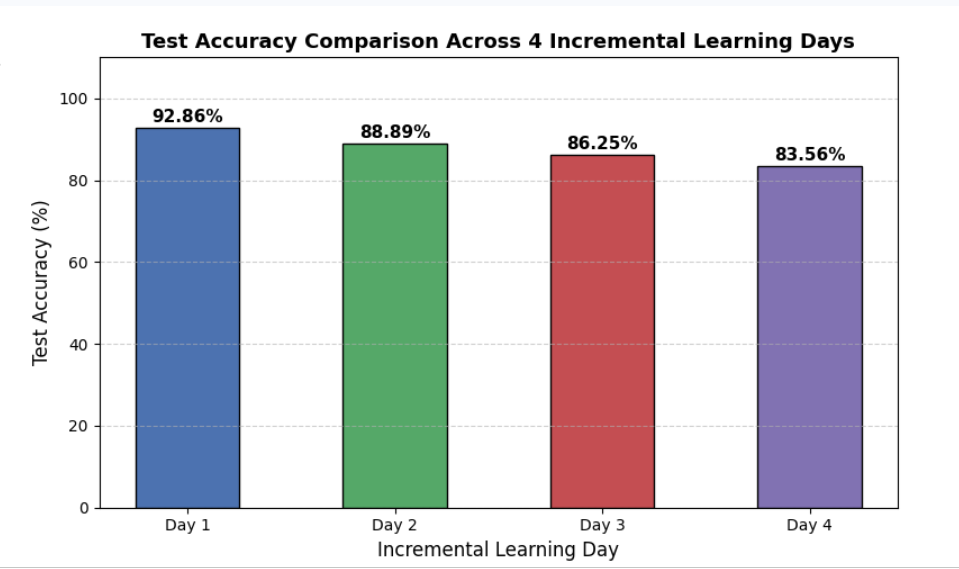
\includegraphics[width=\linewidth]{images/overall_result_chart.png}
\caption{Test Accuracy Comparison Across Four Incremental Learning Days}
\label{fig:test_accuracy_incremental}
\end{figure}

With an increasingly larger dataset that increased from 700 to 1,123 samples over the course of the incremental learning process, the ELM's average test accuracy on all four incremental days was 87.89\%, correctly classifying all five categories of social engineering attacks: baiting, legitimate, phishing, pretexting, and whaling. DAIL augmentation was also found to be a successful method for information retention in the system, as no previously acquired class was completely forgotten during the incremental learning process. % IMPLEMENTATION
%-----------------------------------------
% Chapter 4 - Social Impact and Sustainability
%-----------------------------------------

\chapter{SOCIAL IMPACT AND SUSTAINABILITY}

\section{SOCIAL IMPACT}

The proposed system has a great social impact as it shields individual users from social engineering attacks that target human trust, urgency, and authority instead of technical vulnerabilities. Such attacks include phishing, baiting, pretexting, whaling, and malicious URL attacks, which often lead to financial loss, identity theft, and unauthorized access to accounts. Many of these attacks go unnoticed until a great deal of damage has been done. The system will act as a smart first line of defense that runs continuously in the background, making it unnecessary for users to have advanced knowledge of cybersecurity. This is particularly important for senior citizens, students, and first-time internet users who are more prone to deceptive digital communication.

In addition to the personal security feature, the system enhances the overall cybersecurity of organizations and fosters digital trust. Social engineering attacks against executives and employees can result in fraudulent transactions, breaches of data, and reputation damage. With strong detection performance on all five attack classes, including strong recall on Whaling and strong F1-score on Pretexting in the incremental learning settings, the system assists in early threat detection, lowering the cost of response, and enhancing regulatory compliance. Furthermore, by leveraging open-source technologies and running efficiently on commodity hardware, the system assists in the democratization of cybersecurity, allowing small businesses, institutions of learning, and NGOs to benefit from cutting-edge cybersecurity protection.

\section{SUSTAINABILITY}

The proposed system is computationally efficient and sustainable. The Extreme Learning Machine calculates the output weights analytically without the need for iterative gradient descent computation, thus eliminating the need for GPU-intensive training. The Stacked Autoencoder is trained only once on the initial data and is left frozen for the rest of the incremental updates, thus eliminating the need for repeated deep learning training cycles. Furthermore, the Fuzzy-PGFDG feature calculations are performed through efficient matrix calculations that can be performed on standard CPU hardware. This is a significant move towards energy efficiency compared to the transformer model or the large language model approach.

Sustainability is further improved by the use of incremental adaptability and memory-efficient design. Unlike conventional machine learning systems, which have to be completely retrained when new types of attacks are discovered, the proposed incremental learning approach incorporates new knowledge without forgetting previously gained knowledge. This increases the useful life of the system. The memory cleanup protocol ensures that old feature matrices and models are deleted after each incremental learning update, regardless of the age of the system. This ensures that the system is scalable without increasing hardware costs, thus improving economic and environmental sustainability. % CONCLUSION AND FUTURE WORK
% Chapter 6

\chapter{CONCLUSION AND FUTURE WORK}\label{cha:conclusion}

\section{CONCLUSION}

This project set out to let the payload decide the route. Existing multi-objective UAV
planners build good Pareto fronts and then choose from them with a rule that knows
nothing about the cargo, or with weights an expert re-tunes for every mission. We
separated the two problems. Tier~1 builds an exact NAMOA* front over a
three-dimensional, wind-aware airspace lattice once per region and weather window, and
stores it with what is needed to tell when it has gone stale. Tier~2 turns four payload
tags into objective weights with an explicit formula, scores every route on the front
and returns the best one, or a HOLD when the weather or the battery rules the mission
out. The chosen route is exported as an ArduPilot mission and has been flown in SITL and
in a Gazebo city world.

The first results are encouraging, with clear caveats. The Tier~1 front was exact in
every benchmark scenario, while MOPSO found 38 of 115 routes on the largest. On that
front the four reference payloads received four different routes, three of them
non-extreme, in about 0.14\,ms each. Wind direction alone moved the energy of the
cheapest route by 27.5\% at a fixed speed, and in SITL the flown track stayed within
0.13\,m RMS of the plan. On the other hand, under a steady wind the front shrank and the
presets collapsed onto two routes, MOPSO ran at reduced settings, the ablation used
fixture data, and the risk weights and battery constants are still placeholders.

\section{FUTURE WORK}

The rest of Phase~I is a set of passes through the evaluation cycle. We will run the
full benchmark (four graphs, nine wind cases, MOPSO at 100 particles, 200 iterations and
30 repetitions) with per-repetition statistics and a significance test; fix the density
labels and the monotonicity grouping; study why the front collapses under steady wind,
testing other normalisations and weight multipliers; repeat the ablation and Tier~2
studies on live map data; compare Tier~2 with crowding distance, knee point, shortest
route and fixed weights over all 225 tag combinations; close the two dashboard defects;
and reduce the Tier~1 runtime on large graphs. On the simulation side, wind will be added
to the Gazebo world, the battery model will be calibrated per payload weight class, and
each preset will be flown under several wind cases with all flight metrics logged.

Phase~II moves the system onto a Pixhawk-equipped F450 quadcopter with a Raspberry
Pi~5 companion computer and a servo payload release. Tier~2 will run on board, and
outdoor flights will measure route adherence and the time from tag entry to mission
start. Further out, the two-tier idea could extend to several drones sharing one front,
to multi-drop routes and to in-flight replanning when the weather changes faster than
the refresh window.


\addtotoc{REFERENCES}
\begin{thebibliography}{99}

\bibitem{ref6}
N.~Altwaijry \textit{et al.}, ``Advancing phishing email detection: A comparative study of deep learning techniques,'' \textit{PLoS One}, vol.~19, no.~3, p.~e0299216, Mar.~2024.

\bibitem{ref17}
N.~Alsufyani and A.~Alzahrani, ``Social engineering attack detection using machine learning,'' \textit{International Journal of Advanced Computer Science and Applications}, vol.~13, no.~2,2022.

\bibitem{ref4}
S.~Ariyadasa, S.~Fernando, and S.~Fernando, ``Detecting phishing attacks using a combined model of LSTM and CNN,'' \textit{Int. J. of Advanced and Applied Sciences}, vol.~7, no.~7, pp.~56--67, 2020.

\bibitem{ref19}
S.~Bagui, D.~Nandi, S.~Bagui, and R.~J.~White, 
``Machine learning and deep learning for phishing email classification using one-hot encoding,'' 
\textit{Journal of Computer Science}, vol.~17, pp.~610--623, 2021, doi:\url{https://doi.org/~10.3844/jcssp.2021.610.623}

\bibitem{ref13}
S.~Bahadoripour, H.~Karimipour, A.~N.~Jahromi, and A.~Islam, ``An explainable multi-modal model for advanced cyber-attack detection in industrial control systems,'' \textit{Internet of Things}, vol.~26, p.~101213, 2024.

\bibitem{ref18}
S.~Gupta, S.~Jain, V.~Awasthi, A.~Sabharwal, M.~Kumar, A.~Gaur, and W.~M.~Khan, 
``Detection of phishing URL based on text feature extraction,'' 
\textit{International Journal of Food and Nutritional Sciences (IJFANS)}, 
vol.~11, Special Issue~6, pp.~465, 2022.

\bibitem{ref10}
``Multi-modal fusion for anomaly detection in cybersecurity: Integrating NLP with network traffic data and system logs,'' \textit{EasyChair Preprint}, 2024.

\bibitem{ref11}
``Multi-modal data fusion techniques for improved cybersecurity threat detection and prediction,'' \textit{Baltic Journal of Modern Learning}, Dec.~2024.

\bibitem{ref7}
S.~Jesmithaa and A.~P.~Eliyas, ``Detecting phishing attacks using convolutional neural network and LSTM,'' in \textit{Proc. 3rd Int. Conf. on Advance Computing and Innovative Technologies in Engineering (ICACITE)}, Greater Noida, India, 2023, pp.~802--807.

\bibitem{ref2}
M.~Lansley, S.~Kapetanakis, and N.~Polatidis, ``SEADer++ v2: Detecting social engineering attacks using natural language processing and machine learning,'' in \textit{Proc. 2020 Int. Conf. on Innovations in Intelligent Systems and Applications (INISTA)}, 2020, pp.~1--6.

\bibitem{ref5}
S.~Madhusudhanan and S.~Jaganathan, ``Data augmented incremental learning (DAIL) for unsupervised data,'' \textit{IEICE Transactions on Information and Systems}, vol.~105, no.~6, pp.~1185--1197, 2022.

\bibitem{ref20}
A.~Mahdieh Zabihimayvan, B.~Derek Doran, 
``Fuzzy rough set feature selection to enhance phishing detection,'' 
\textit{arXiv preprint arXiv:1903.05675}, 2019.

\bibitem{ref16}
A.~Namavar~Jahromi \textit{et al.}, ``A deep multi-modal cyber-attack detection model,'' \textit{arXiv preprint arXiv:2304.01440}, 2023.

\bibitem{ref8}
M.~K.~Prabakaran, P.~M.~Sundaram, and A.~D.~Chandrasekar, ``An enhanced deep learning-based phishing detection mechanism to effectively identify malicious URLs using variational autoencoders,'' \textit{IET Information Security}, vol.~17, pp.~423--440, 2023.

\bibitem{ref3}
A.~Prasad and S.~Chandra, ``PhiUSIIL: A diverse security profile empowered phishing URL detection framework based on similarity index and incremental learning,'' \textit{Computers \& Security}, vol.~136, p.~103539, 2024.

\bibitem{ref9}
O.~K.~Sahingoz, E.~Buber, and O.~Kugu, ``A dual-phase deep learning framework for advanced phishing detection using multiple algorithms,'' \textit{Scientific Reports}, vol.~15, p.~21986, Jul.~2025.

\bibitem{ref21}
B.~Senthilnayaki, K.~Venkatalakshmi, and A.~Kannan, 
``Intrusion detection system using fuzzy rough set feature selection and modified KNN classifier,'' 
\textit{The International Arab Journal of Information Technology}, 
vol.~16, no.~4, Jul.~2019.

\bibitem{ref15}
M.~S.~V.~Tyagadurgam \textit{et al.}, ``Preventing phishing attacks using advanced deep learning techniques for cyber threat mitigation,'' \textit{Journal of Data Analysis and Information Processing}, vol.~13, pp.~314--330, 2025.

\bibitem{ref12}
C.~Xu, Y.~Zhan, Z.~Wang, and J.~Yang, ``Multimodal fusion based few-shot network intrusion detection system,'' \textit{Scientific Reports}, vol.~15, p.~21986, Jul.~2025.

\bibitem{ref14}
Y.~Zhang \textit{et al.}, ``Detection and classification of phishing websites using machine learning,'' \textit{Cybersecurity}, vol.~8, no.~1, pp.~1--18, May~2025.

\bibitem{ref1}
P.~Vidyasri and S.~Suresh, ``FDN-SA: Fuzzy deep neural-stacked autoencoder-based phishing attack detection in social engineering,'' \textit{Computers \& Security}, vol.~148, p.~104188, 2025.

\end{thebibliography}

\end{spacing}
\end{document}
`
